\documentclass{article}

% if you need to pass options to natbib, use, e.g.:
%     \PassOptionsToPackage{numbers, compress}{natbib}
% before loading neurips_2019

% ready for submission
 \usepackage{neurips_2019}

% to compile a preprint version, e.g., for submission to arXiv, add add the
% [preprint] option:
%     \usepackage[preprint]{neurips_2019}

% to compile a camera-ready version, add the [final] option, e.g.:
%     \usepackage[final]{neurips_2019}

% to avoid loading the natbib package, add option nonatbib:
%     \usepackage[nonatbib]{neurips_2019}

\usepackage[utf8]{inputenc} % allow utf-8 input
\usepackage[T1]{fontenc}    % use 8-bit T1 fonts
\usepackage{hyperref}       % hyperlinks
\usepackage{url}            % simple URL typesetting
\usepackage{booktabs}       % professional-quality tables
\usepackage{amsfonts}       % blackboard math symbols
\usepackage{nicefrac}       % compact symbols for 1/2, etc.
\usepackage{microtype}      % microtypography

\usepackage[T1]{fontenc}    % use 8-bit T1 fonts
\usepackage{hyperref}       % hyperlinks
\usepackage{url}            % simple URL typesetting
\usepackage{booktabs}       % professional-quality tables
\usepackage{amsfonts}       % blackboard math symbols
\usepackage{nicefrac}       % compact symbols for 1/2, etc.
\usepackage{wrapfig}
\usepackage{picins}

\usepackage[backgroundcolor = White,textwidth=2cm]{todonotes}
%\usepackage[disable,backgroundcolor = White,textwidth=\marginparwidth]{todonotes}
\newcommand{\todom}[2][]{\todo[color=orange!25,size=\small,#1]{G: #2}}
\newcommand{\todox}[2][]{\todo[color=purple!25,size=\small,#1]{K: #2}}
\newcommand{\todor}[2][]{\todo[color=blue!25,size=\small,#1]{R: #2}}
\setlength{\marginparwidth}{0.8in}

% Set the typeface to Times Roman
\usepackage{times}

\usepackage{algorithm,algorithmic}
%\newcommand{\theHalgorithm}{\arabic{algorithm}}

\usepackage{microtype}
\usepackage{graphicx}
\usepackage{subfigure}
\usepackage{booktabs} % for professional tables

\usepackage{natbib}

\usepackage{amssymb,amsmath,amsthm} %maths
\usepackage{hyperref}
\usepackage[utf8]{inputenc} %useful to type directly diacritic characters
\usepackage[capitalize]{cleveref}

\crefname{prop}{Proposition}{Propositions}
\crefname{thm}{Theorem}{Theorems}
\crefname{lem}{Lemma}{Lemmas}
\crefname{algorithm}{Algorithm}{Algorithms}

\def\rva{{\mathbf{a}}}
\def\rvo{{\mathbf{o}}}
\def\rvr{{\mathbf{r}}}
\def\rvs{{\mathbf{s}}}
\def\rvu{{\mathbf{u}}}
\def\rvw{{\mathbf{w}}}
\def\rvx{{\mathbf{x}}}
\def\rvg{{\mathbf{g}}}
\def\rvo{{\mathbf{o}}}
\def\rvone{{\mathbf{1}}}
\def\rvzero{{\mathbf{0}}}
\def\rvtilder{{\tilde{\mathbf{r}}}}
\def\rvhat{{\hat{\mathbf{r}}}}

\def\rvp{{\mathbf{p}}}

\def\pr{{\text{Pr}}}
\def\r{{\text{R}}}

\def\ucb{{\text{U}}}
\def\lcb{{\text{L}}}

\newtheorem{thm}{Theorem}
\newtheorem{lem}{Lemma}
\newtheorem{defi}{Definition}
\newtheorem{prop}{Proposition}
\newtheorem{remk}{Remark}

\def\rvpi{{\boldsymbol{\pi}}}

\def\rmA{{\mathbf{A}}}
\def\rmD{{\mathbf{D}}}
\def\rmH{{\mathbf{H}}}
\def\rmI{{\mathbf{I}}}
\def\rmW{{\mathbf{W}}}
\def\rmX{{\mathbf{X}}}

\def\sE{{\mathbb{E}}}
\def\sR{{\mathbb{R}}}
\def\sI{{\mathbb{I}}}
\def\sP{{\mathbb{P}}}

\def\gN{{\mathcal{N}}}
\def\gE{{\mathcal{E}}}
\def\gU{{\mathcal{U}}}

\DeclareMathOperator*{\argmax}{arg\,max}
\DeclareMathOperator*{\argmin}{arg\,min}
\DeclareMathOperator*{\probability}{Pr}
\DeclareMathOperator*{\expectation}{\sE}
\DeclareMathOperator*{\trace}{Tr}


\renewcommand{\algorithmicrequire}{\textbf{Input:}}
\renewcommand{\algorithmicensure}{\textbf{Output:}}

\title{Appendix of ``Provable Reinforcement Learning Algorithms with Neural Networks on Stochastic Multi-Armed Bandit''}

% The \author macro works with any number of authors. There are two commands
% used to separate the names and addresses of multiple authors: \And and \AND.
%
% Using \And between authors leaves it to LaTeX to determine where to break the
% lines. Using \AND forces a line break at that point. So, if LaTeX puts 3 of 4
% authors names on the first line, and the last on the second line, try using
% \AND instead of \And before the third author name.

\author{%
  David S.~Hippocampus\thanks{Use footnote for providing further information
    about author (webpage, alternative address)---\emph{not} for acknowledging
    funding agencies.} \\
  Department of Computer Science\\
  Cranberry-Lemon University\\
  Pittsburgh, PA 15213 \\
  \texttt{hippo@cs.cranberry-lemon.edu} \\
  % examples of more authors
  % \And
  % Coauthor \\
  % Affiliation \\
  % Address \\
  % \texttt{email} \\
  % \AND
  % Coauthor \\
  % Affiliation \\
  % Address \\
  % \texttt{email} \\
  % \And
  % Coauthor \\
  % Affiliation \\
  % Address \\
  % \texttt{email} \\
  % \And
  % Coauthor \\
  % Affiliation \\
  % Address \\
  % \texttt{email} \\
}

\begin{document}

\maketitle

\appendix

\section{Proofs of Policy Gradient}

This section contains the detailed proofs of \cref{thm_appendix:policy_gradient_main_result} and the related technical lemmas.

\subsection{Proof of \cref{thm_appendix:policy_gradient_main_result}}

For convenience, we restate \cref{thm_appendix:policy_gradient_main_result} here.

\begin{thm}
	\label{thm_appendix:policy_gradient_main_result}
	Given policy neural networks as shown in \cref{fig:nn_policy_value}, with number of parameters $m \ge \frac{T^2}{h^2}$, $\eta = \frac{1}{2 h m}$, $\beta = \frac{ \ln{\left(\frac{h}{3}\right) + \ln{\ln{t}} } }{ 3 \ln{t}}$, the expected regret of \cref{alg:policy_gradient_uniform_exploration} satisfies,
	\begin{equation*}
	\begin{split}
	\sum\limits_{t=0}^{T-1}{ \left( {\rvpi^*}^\top \rvr - \sE \left[ r\left(A_t\right) \right] \right)} \le O\left(T^{\frac{2}{3}}\left( \ln{T} \right)^{\frac{1}{3}}\right).
	\end{split}
	\end{equation*}
\end{thm}
\begin{proof}
    According to \cref{alg:policy_gradient_uniform_exploration}, $\tilde{\rvpi}_t$ is used for sampling, which is $\rvpi\left( \rmW_t \right)$ mixed with decaying uniform. Therefore the regret is divided by the linearity of the expectation.
\begin{equation}
\label{eq:total_regret_decomposition}
\begin{split}
    \sum\limits_{t=0}^{T-1}{ \left( {\rvpi^*}^\top \rvr - \sE \left[ r\left(A_t\right) \right] \right) } &\le 1 + \sum\limits_{t=1}^{T-1}{ \left[ \left( 1 - t^{ \beta - \frac{1}{3}} \right) \cdot \left( {\rvpi^*} - \rvpi\left( \rmW_t \right) \right)^\top \rvr + t^{ \beta - \frac{1}{3}} \cdot \left( {\rvpi^*}^\top \rvr - \expectation\limits_{A_t \sim \unif[h]}{ \left[ r\left(A_t\right) \right] } \right) \right]} \\
    &\le 1 + \sum\limits_{t=1}^{T-1}{ \left[ \left( {\rvpi^*} - \rvpi\left( \rmW_t \right) \right)^\top \rvr + t^{ \beta - \frac{1}{3}} \right]} \\
    &\le 1 + \sum\limits_{t=1}^{T-1}{ \left( \frac{ h \ln{t} }{t} \right)^{\frac{1}{3}} } + \sum\limits_{t=1}^{T-1}{ \left( {\rvpi^*} - \rvpi\left( \rmW_t \right) \right)^\top \rvr } \\
    &\le 2 \cdot T^{\frac{2}{3}} \cdot \left( h \ln{T} \right)^{\frac{1}{3}} + \sum\limits_{t=1}^{T-1}{ \left( {\rvpi^*} - \rvpi\left( \rmW_t \right) \right)^\top \rvr },
\end{split}
\end{equation}
where the second inequality comes from $1 - t^{ \beta - \frac{1}{3}} \le 1$, $\forall t \ge 1$, and $\left\| \rvr \right\|_\infty \le 1$, and the third inequality is according to the value of $\beta$. Denote $\rvpi_t^* \triangleq \argmax\limits_{\rvpi \in \Delta^{h-1}}{\left\{ \rvpi^\top \hat{\rvr}_t\right\}}$. The last term can be decomposed as follows, $\forall t \ge 1$,
\begin{equation}
\label{eq:playing_learning_phase_regret_decomposition}
\begin{split}
    \left( {\rvpi^*} - \rvpi\left( \rmW_t \right) \right)^\top \rvr &= \left( {\rvpi^*} - {\rvpi_t^*} \right)^\top \hat{\rvr}_t + \left( {\rvpi_t^*} - \rvpi\left( \rmW_t \right) \right)^\top \hat{\rvr}_t + \left( {\rvpi^*} - \rvpi\left( \rmW_t \right) \right)^\top \left( \rvr - \hat{\rvr}_t \right) \\
    &\le \left( {\rvpi_t^*} - \rvpi\left( \rmW_t \right) \right)^\top \hat{\rvr}_t  + \left\| \rvpi^* - \rvpi\left( \rmW_t \right) \right\|_1 \cdot \left\| \rvr - \hat{\rvr}_t \right\|_\infty \\
    &\le \left( {\rvpi_t^*} - \rvpi\left( \rmW_t \right) \right)^\top \hat{\rvr}_t  + 2 \cdot \left\| \rvr - \hat{\rvr}_t \right\|_\infty,
\end{split}
\end{equation}
where the first inequality is by the definition of $\rvpi_t^*$ and  H{\"o}lder's inequality. Next, we prove several events happen with high probabilities. Define
\begin{equation*}
    \gE_1 \triangleq \left\{ \left\| \hat{\rvr}_t - \rvr \right\|_\infty \le t^{\beta - \frac{1}{3}} \le \left( h \ln{t} \right) ^\frac{1}{3} \cdot t^{- \frac{1}{3}}, \quad \forall t \ge \frac{h}{3} \ln{\left(\frac{h}{3}\right) } \right\}.
\end{equation*}

According to \cref{thm:reward_estimation_hoeffding}, we have 
\begin{equation*}
    \pr\left\{ \gE_1 \right\} \ge
    1 - h \cdot \exp\left\{ - \frac{t^{\frac{1}{3}}}{2 h^2} \cdot \left( \frac{h}{3} \ln{t} \right)^{\frac{2}{3}} \right\} - 2 h \cdot t^{- \frac{1}{3}}.
\end{equation*}
Therefore we have the last term in \cref{eq:playing_learning_phase_regret_decomposition} satisfies,
\begin{equation}
\label{eq:estimation_upper_bound}
\begin{split}
    2 \cdot \sum\limits_{t=1}^{T-1}{ \left\| \rvr - \hat{\rvr}_t \right\|_\infty } &\le \frac{2 h}{3} \ln{\left(\frac{h}{3}\right) } + \underbrace{2 \cdot \sum\limits_{t=1}^{T-1}{ \left( h \ln{t} \right) ^\frac{1}{3} \cdot t^{- \frac{1}{3}} }}_{\gE_1 \text{ happens, } \pr\left\{ \gE_1 \right\} \le 1} + \underbrace{ 2 \cdot  \sum\limits_{t=1}^{T-1}{ \left[ h \cdot \exp\left\{ - \frac{t^{\frac{1}{3}}}{2 h^2} \cdot \left( \frac{h}{3} \ln{t} \right)^{\frac{2}{3}} \right\} + 2 h \cdot t^{- \frac{1}{3}} \right] } }_{ \gE_1 \text{ does not happen, } \left\| \rvr - \hat{\rvr}_t \right\|_\infty \le 1 } \\
    &\le \frac{2 h}{3} \ln{\left(\frac{h}{3}\right) } + 3 \cdot T^{\frac{2}{3}} \cdot \left( h \ln{T} \right) ^\frac{1}{3} + 6 \cdot h \cdot T^{\frac{2}{3}} + o(1) \\
    &\le h \ln{h} + 3 \cdot T^{\frac{2}{3}} \cdot \left( h \ln{T} \right) ^\frac{1}{3} + 6 \cdot h \cdot T^{\frac{2}{3}}.
\end{split}
\end{equation}

It remains to bound the summation of the ``dynamic regret'' $\left( {\rvpi^*} - \rvpi\left( \rmW_t \right) \right)^\top \rvr$ in \cref{eq:playing_learning_phase_regret_decomposition}. Define
\begin{equation*}
    \gE_2 \triangleq \left\{ \sum\limits_{t=1}^{T-1}{ \left(  {\rvpi_t^*} - \rvpi\left( \rmW_t \right) \right)^\top \hat{\rvr}_t } \le \frac{7 h}{c} \cdot  T^{\frac{2}{3}}, \quad c \in O(1) \right\}.
\end{equation*}

According to \cref{thm:dynamic_regret_sublinear}, we have,
\begin{equation*}
    \pr\left\{ \gE_2 \right\} \ge 1 - \exp\left\{ - \frac{T^2}{16 h^2} \right\} \ge 1 - \frac{16 h^2}{T^2}.
\end{equation*}

Therefore we have the dynamic regret in \cref{eq:playing_learning_phase_regret_decomposition} satisfies,
\begin{equation}
\label{eq:dynamic_regret_upper_bound}
\begin{split}
    \sum\limits_{t=1}^{T-1}{ \left(  {\rvpi_t^*} - \rvpi\left( \rmW_t \right) \right)^\top \hat{\rvr}_t } &\le \underbrace{ \frac{7 h}{c} \cdot  T^{\frac{2}{3}} }_{ \gE_2 \text{ happens}} + \underbrace{ \frac{16 h}{T^2} \cdot T }_{ \gE_2 \text{ does not happen}} \\
    &\le \frac{8 h}{c} \cdot  T^{\frac{2}{3}}.
\end{split}
\end{equation}

Finally, combining all the results \cref{eq:total_regret_decomposition}, \cref{eq:playing_learning_phase_regret_decomposition}, \cref{eq:estimation_upper_bound}, and \cref{eq:dynamic_regret_upper_bound}, we have,
\begin{equation*}
\begin{split}
    \sum\limits_{t=0}^{T-1}{ \left( {\rvpi^*}^\top \rvr - \sE \left[ r\left(A_t\right) \right] \right) } &\le 2 \cdot T^{\frac{2}{3}} \cdot \left( h \ln{T} \right)^{\frac{1}{3}} + h \ln{h} + 3 \cdot T^{\frac{2}{3}} \cdot \left( h \ln{T} \right) ^\frac{1}{3} + 6 \cdot h \cdot T^{\frac{2}{3}} + \frac{8 h}{c} \cdot  T^{\frac{2}{3}} \\
    &\le 5 \cdot T^{\frac{2}{3}} \cdot \left( h \ln{T} \right)^{\frac{1}{3}} + \frac{9 h}{c} \cdot  T^{\frac{2}{3}} + h \ln{h} \\
    &\le O\left(T^{\frac{2}{3}}\left( \ln{T} \right)^{\frac{1}{3}}\right). \qedhere
\end{split}
\end{equation*}
\end{proof}

\begin{thm}
\label{thm:reward_estimation_hoeffding}
    In \cref{alg:policy_gradient_uniform_exploration}, let $\beta = \frac{ \ln{\left(\frac{h}{3}\right) + \ln{\ln{t}} } }{ 3 \ln{t}}$, we have,
\begin{equation*}
    \left\| \hat{\rvr}_t - \rvr \right\|_\infty \le t^{\beta - \frac{1}{3}} \le \left( h \ln{t} \right) ^\frac{1}{3} \cdot t^{- \frac{1}{3}}, \quad \forall t \ge \frac{h}{3} \ln{\left(\frac{h}{3}\right) },
\end{equation*}
with probability at least,
\begin{equation*}
    1 - h \cdot \exp\left\{ -  \frac{t^{\frac{1}{3} + 2 \beta}}{2 h^2} \right\} - 2 h \cdot \exp\left\{ - \frac{t^{3\beta}}{ h } \right\} = 1 - h \cdot \exp\left\{ - \frac{t^{\frac{1}{3}}}{2 h^2} \cdot \left( \frac{h}{3} \ln{t} \right)^{\frac{2}{3}} \right\} - 2 h \cdot t^{- \frac{1}{3}}.
\end{equation*}
\end{thm}
\begin{proof}
    Denote $\tilde{n}_t(k) \triangleq \sum\limits_{s=0}^{t}{ \tilde{\pi}_t(k)}$, which can be lower bounded as,
\begin{equation*}
\begin{split}
    \tilde{n}_t(k) &\ge \sum\limits_{s=1}^{t}{ \tilde{\pi}_t(k)} = \sum\limits_{s=1}^{t}{ \left[ \left( 1 - s^{\beta - \frac{1}{3}} \right) \cdot \pi\left(\rmW_{s}\right)(k) + \frac{s^{\beta - \frac{1}{3}}}{h} \right] } \\
    &\ge \sum\limits_{s=1}^{t}{ \frac{s^{\beta - \frac{1}{3}}}{h} } \ge \frac{t^{\frac{2}{3} + \beta}}{ h  \left(\frac{2}{3} + \beta \right) } \ge \frac{t^{\frac{2}{3} + \beta}}{ h },
\end{split}
\end{equation*}
where the last inequality is by $\beta \le \frac{1}{3}$, $\forall t \ge \frac{h}{3} \ln{\left(\frac{h}{3}\right) }$. According to Theorem 2.3 in \citep{wainwright2015mathematical} or \citep{wainwright2019high},
\begin{equation*}
\begin{split}
    \pr\left\{ n_t(k) - \tilde{n}_t(k) < - a \right\} \le \exp\left\{ - \frac{a^2}{2 \sum_{s=1}^{t}{\sigma_s^2} } \right\} \le \exp\left\{ - \frac{2 a^2}{ t } \right\},
\end{split}
\end{equation*}
where $\sigma_s \le \frac{1}{4}$ is the variance of $\text{Bernoulli}\left( \tilde{\pi}_t(k) \right)$
Therefore, the following event
\begin{equation*}
    \gE_3 \triangleq \left\{ n_t(k) \ge \tilde{n}_t(k) - \frac{t^{\frac{2}{3} + \beta}}{ 2 h } \ge \frac{t^{\frac{2}{3} + \beta}}{ 2 h }, \forall k \in [h] \right\},
\end{equation*}
holds with probability at least $1 - h \cdot \exp\left\{ -  \frac{t^{\frac{1}{3} + 2 \beta}}{2 h^2} \right\}$. Assume $\gE_3$ happens, according to the Hoeffding's inequality, the following event
\begin{equation*}
    \gE_4 \triangleq \left\{ \left| \hat{r}_{t}(k) - r(k) \right| \le t^{\beta - \frac{1}{3}} , \forall k \in [h] \right\}
\end{equation*}
holds with probability at least $1 - 2 h \cdot \exp\left\{ - \frac{t^{3\beta}}{ h } \right\}$.
\end{proof}

\begin{thm}
\label{thm:dynamic_regret_sublinear}
    If $m \ge \frac{T^2}{h^2}$, $\eta = \frac{1}{2 h m}$, then the dynamic regret satisfies,
\begin{equation*}
\begin{split}
    \sum\limits_{t=1}^{T-1}{ \left(  {\rvpi_t^*} - \rvpi\left( \rmW_t \right) \right)^\top \hat{\rvr}_t } \le \frac{5 h}{c} \cdot  T^{\frac{2}{3}},
\end{split}
\end{equation*}
with probability at least $1 - \exp\left\{ - \frac{T^2}{16 h} \right\} \ge 1 - \frac{16 h}{T^2}$.
\end{thm}
\begin{proof}
    Denote $\delta_t \triangleq \left( {\rvpi_t^*} - \rvpi\left( \rmW_t \right) \right)^\top \hat{\rvr}_t$. Decompose $\delta_t$ as follows,
\begin{equation}
\label{eq:dynamic_regret_decomposition}
\begin{split}
    \delta_t &= {\rvpi_t^*}^\top \left( \hat{\rvr}_t - \hat{\rvr}_{t-1}\right) + \left( {\rvpi_t^*} - {\rvpi_{t-1}^*} \right)^\top \hat{\rvr}_{t-1}  + \left( {\rvpi_{t-1}^*} - \rvpi\left( \rmW_{t-1} \right) \right)^\top \hat{\rvr}_{t-1} \\
    &\quad + \left(  \rvpi\left( \rmW_{t-1} \right) - \rvpi\left( \rmW_t \right) 
    \right)^\top \hat{\rvr}_{t-1} + \rvpi\left( \rmW_t \right)^\top \left( \hat{\rvr}_{t-1} - \hat{\rvr}_t \right).
\end{split}
\end{equation}
We upper bound each term in the right hand side. Firstly,
\begin{equation*}
\begin{split}
    {\rvpi_t^*}^\top \left( \hat{\rvr}_t - \hat{\rvr}_{t-1}\right) &= \frac{\pi_{t}^*\left(A_{t-1}\right)}{n_{t}\left(A_{t-1}\right)} \left[ R_{ A_{t-1}}\left( n_{t}\left(A_{t-1}\right) -1 \right) - \hat{r}_{t-1}\left(A_{t-1}\right) \right] \\
    &\le \frac{1}{n_{t}\left(A_{t-1}\right)} \le \frac{ 2 h }{t^{\frac{2}{3} + \beta}},
\end{split}
\end{equation*}
by $n_{t}\left(A_{t-1}\right) = n_{t-1}\left(A_{t-1}\right) + 1$, and $n_{t}\left(A_{t-1}\right) \ge \frac{t^{\frac{2}{3} + \beta}}{ 2 h }$, $\forall t \ge 1$. By the definition of ${\rvpi_{t-1}^*}$,
\begin{equation*}
    \left( {\rvpi_t^*} - {\rvpi_{t-1}^*} \right)^\top \hat{\rvr}_{t-1} \le 0.
\end{equation*}
Note that according to the definition of $\delta_t$,
\begin{equation*}
    \left( {\rvpi_{t-1}^*} - \rvpi\left( \rmW_{t-1} \right) \right)^\top \hat{\rvr}_{t-1} = \delta_{t-1}.
\end{equation*}
By \cref{lem:gradient_coupling}, \cref{lem:empirically_expected_reward_parameter_smoothness}, $\eta = \frac{1}{2 h m}$, and \cref{lem:gradient_lower_bound},
\begin{equation*}
\begin{split}
    &\left( \rvpi\left( \rmW_{t-1} \right) - \rvpi\left( \rmW_t \right) \right)^\top \hat{\rvr}_{t-1} \le - \frac{1}{4 h m} \left\| \frac{d \rvpi\left( \rmW_{t-1} \right)^\top \hat{\rvr}_{t-1}}{d \rmW_{t-1}} \right\|_F^2 \\
    &\quad = - \frac{1}{4 h m} \sum\limits_{r=1}^{m}{ \left\| \frac{d \rvpi\left( \rmW_{t-1} \right)^\top \hat{\rvr}_{t-1}}{d \rvw_r(t-1)} \right\|_2^2 } \le - \frac{c^2}{4 h} \left[ \left( {\rvpi_{t-1}^*} - \rvpi\left( \rmW_{t-1} \right) \right)^\top \hat{\rvr}_{t-1}  \right]^2 = - \frac{c^2}{4 h} \cdot \delta_{t-1}^2.
\end{split}
\end{equation*}
Using similar arguments,
\begin{equation*}
    \rvpi\left( \rmW_t \right)^\top \left( \hat{\rvr}_{t-1} - \hat{\rvr}_t  \right) \le \frac{ 2 h }{t^{\frac{2}{3} + \beta}}.
\end{equation*}
Plugging the above upper bounds into \cref{eq:dynamic_regret_decomposition},
\begin{equation*}
    \delta_t \le \delta_{t-1} - \frac{c^2}{4 h} \cdot \delta_{t-1}^2 + \frac{ 4 h }{t^{\frac{2}{3} + \beta}}.
\end{equation*}
Rearranging and summing up from $1$ to $T-1$,
\begin{equation*}
\begin{split}
    \sum\limits_{t=1}^{T-1}{\delta_{t}^2} = \sum\limits_{t=2}^{T}{\delta_{t-1}^2} \le \frac{4 h}{ c^2} \cdot  \sum\limits_{t=2}^{T} { \left[ \delta_{t-1} - \delta_t + \frac{ 4 h }{t^{\frac{2}{3} + \beta}} \right] } \le \frac{49 h^2}{ c^2} \cdot T^{\frac{1}{3}}.
\end{split}
\end{equation*}
By the Root-Mean Square-Arithmetic Mean inequality,
\begin{equation*}
\begin{split}
    \sum\limits_{t=1}^{T-1}{\delta_{t}} \le \sqrt{\left(T  - 1 \right) \cdot \sum\limits_{t=1}^{T-1}{\delta_{t}^2}} \le \frac{7 h}{c} \cdot  T^{\frac{2}{3}}.
\end{split}
\end{equation*}
Let $\sigma = \frac{2 \sqrt{2}}{\sqrt{\pi m}}$ and $\tau = \frac{\sigma \sqrt{\pi}}{2 \sqrt{2}} = \frac{1}{\sqrt{m}}$ in \cref{lem:gradient_coupling}. Since $m \ge \frac{T^2}{h^2}$, we have $T \le \frac{\tau}{2 \eta}$ such that \cref{lem:gradient_coupling} holds during all the $T$ steps. According to \cref{lem:gradient_coupling_in_total}, with probability at least $1 - \exp\left\{ - \frac{m}{8} \left( 1 - \frac{\sqrt{2}\tau}{\sqrt{\pi}\sigma} \right) \right\} = 1 - \exp\left\{ - \frac{m}{16} \right\} \ge 1 - \exp\left\{ - \frac{T^2}{16 h^2} \right\}$ over the random initialization of the neural networks, all the intermediately used lemmas hold, therefore the results hold.
\end{proof}

\subsection{Proof of Lemmas Supporting \cref{thm:dynamic_regret_sublinear}}

\cref{thm:dynamic_regret_sublinear} relies on two arguments. First, the dynamic expected loss is smooth in the logit space, and small policy gradient updates preserve the signs of ReLU outputs, therefore highly correlates the logit derivative and the policy gradient. Second, by the over-parameterization theory, gradient norm is lower bounded by expected loss around initialization, which means there is no bad local minima near the randomly initialized neural network policy $\rvpi\left( \rmW_0 \right)$.

\begin{lem}
\label{lem:logit_smoothness}
Let $\rvpi(\rvo^\prime)$ and $\rvpi( \rvo)$ be the softmax policies of any logit vectors $\rvo^\prime, \rvo \in \sR^h$, respectively. $\forall \rvr \in \left[ -1, 1\right]^h$,
\begin{equation*}
    \rvpi(\rvo^\prime)^\top \rvr \le \rvpi(\rvo)^\top \rvr + \left\langle \frac{d \rvpi(\rvo)^\top \rvr}{d \rvo}, \rvo^\prime - \rvo \right\rangle + \left\| \rvo^\prime - \rvo \right\|_2^2.
\end{equation*}
\end{lem}
\begin{proof}
Denote $\rvo_{\xi} = \rvo + \xi \left( \rvo^\prime - \rvo \right)$.
\begin{equation*}
\begin{split}
    &\left| \rvpi\left( \rvo^\prime \right)^\top \rvr - \rvpi\left( \rvo \right)^\top \rvr - \left\langle \frac{d \rvpi\left( \rvo \right)^\top \rvr}{d \rvo}, \rvo^\prime - \rvo \right\rangle \right| \\
    &\quad = \left| \int_0^1{ \frac{d \rvpi\left( \rvo + \xi \left( \rvo^\prime - \rvo \right) \right)^\top \rvr}{d \xi} d\xi} - \left\langle \frac{d \rvpi\left( \rvo \right)^\top \rvr}{d \rvo}, \rvo^\prime - \rvo \right\rangle \right| \\
    &\quad = \left| \int_0^1{ \left\langle \frac{d \rvpi\left( \rvo + \xi \left( \rvo^\prime - \rvo \right) \right)^\top \rvr}{d \left( \rvo + \xi \left( \rvo^\prime - \rvo \right) \right)}, \rvo^\prime - \rvo \right\rangle d\xi} - \left\langle \frac{d \rvpi\left( \rvo \right)^\top \rvr}{d \rvo}, \rvo^\prime - \rvo \right\rangle \right| \\
    &\quad = \left| \int_0^1{ \left\langle \frac{d \rvpi\left( \rvo_{\xi} \right)^\top \rvr}{d \rvo_{\xi}} - \frac{d \rvpi\left( \rvo \right)^\top \rvr}{d \rvo}, \rvo^\prime - \rvo \right\rangle d\xi} \right| \\
    &\quad \le \int_0^1{ \left| \left\langle \frac{d \rvpi\left( \rvo_{\xi} \right)^\top \rvr}{d \rvo_{\xi}} - \frac{d \rvpi\left( \rvo \right)^\top \rvr}{d \rvo}, \rvo^\prime - \rvo \right\rangle \right| d\xi} \\
    &\quad \le \int_0^1{ \left\| \frac{d \rvpi\left( \rvo_{\xi} \right)^\top \rvr}{d \rvo_{\xi}} - \frac{d \rvpi\left( \rvo \right)^\top \rvr}{d \rvo} \right\|_2 \cdot \left\| \rvo^\prime - \rvo \right\|_2 d\xi} \\
    &\quad = \int_0^1{ \left\| \rmH\left( \rvpi\left( \rvo_{\xi} \right)\right) \rvr - \rmH\left( \rvpi\left( \rvo \right)\right) \rvr \right\|_2 \cdot \left\| \rvo^\prime - \rvo \right\|_2 d\xi} \\
    &\quad = \int_0^1{ \left\| \int_0^1{\left\langle \frac{d \rmH \left( \rvpi\left( \rvo + \mu\left( \rvo_{\xi} - \rvo \right) \right) \right) \rvr }{d \left( \rvo + \mu\left( \rvo_{\xi} - \rvo \right) \right)}, \rvo_{\xi} - \rvo \right\rangle d\mu} \right\|_2 \cdot \left\| \rvo^\prime - \rvo \right\|_2 d\xi} \\
    &\quad \le \int_0^1{  \int_0^1{ \left\| \left\langle \frac{d \rmH \left( \rvpi\left( \rvo + \mu\left( \rvo_{\xi} - \rvo \right) \right) \right) \rvr }{d \left( \rvo + \mu\left( \rvo_{\xi} - \rvo \right) \right)}, \rvo_{\xi} - \rvo \right\rangle \right\|_2 d\mu} \cdot \left\| \rvo^\prime - \rvo \right\|_2 d\xi} \\
    &\quad \le \int_0^1{  \int_0^1{ \left\| \frac{d \rmH \left( \rvpi\left( \rvo + \mu\left( \rvo_{\xi} - \rvo \right) \right) \right) \rvr }{d \left( \rvo + \mu\left( \rvo_{\xi} - \rvo \right) \right)} \right\|_2 \cdot \left\| \rvo_{\xi} - \rvo \right\|_2 d\mu} \cdot \left\| \rvo^\prime - \rvo \right\|_2 d\xi} \\
    &\quad = \int_0^1{  \int_0^1{ \left\| \frac{d \rmH \left( \rvpi\left( \rvo + \mu\left( \rvo_{\xi} - \rvo \right) \right) \right) \rvr }{d \left( \rvo + \mu\left( \rvo_{\xi} - \rvo \right) \right)} \right\|_2 d\mu} \cdot \xi \cdot \left\| \rvo^\prime - \rvo \right\|_2^2 d\xi} \\
    &\quad \le \int_0^1{  \int_0^1{ 2 d\mu} \cdot \xi \cdot \left\| \rvo^\prime - \rvo \right\|_2^2 d\xi} \\
    &\quad = \left\| \rvo^\prime - \rvo \right\|_2^2,
\end{split}
\end{equation*}
where the last inequality is according to \cref{lem:Hr_spectral_norm_upper_bound}.
\end{proof}

\begin{lem}
\label{lem:Hr_spectral_norm_upper_bound}
    Let $\rvo \in \sR^h$ be any logit vector, and $\rvpi(\rvo)$ be the softmax policy of $\rvo$ at state $\rvs$. Denote $\rmH\left( \rvpi \left(\rvo \right) \right) \triangleq \Delta \left( \rvpi \left(\rvo \right) \right) - \rvpi \left(\rvo \right) \rvpi \left(\rvo \right)^\top$, where $\Delta \left( \rvpi \left(\rvo \right) \right) \in \sR^{h \times h}$ is a matrix with $\rvpi \left(\rvo \right)$ as its diagonal. $\forall \rvr \in \left[ -1, 1\right]^h$,
\begin{equation*}
    \left\| \frac{d \rmH\left( \rvpi \left(\rvo \right) \right) \rvr}{d \rvo } \right\|_2 \le 2,
\end{equation*}
where $\left\| \cdot \right\|_2$ is the matrix spectral norm.
\end{lem}
\begin{proof}
    Denote $\rmS \triangleq \frac{d \rmH\left( \rvpi \left(\rvo \right) \right) \rvr}{d \rvo } \in \sR^{h \times h}$. $\forall s, t \in [h]$,
\begin{equation*}
\begin{split}
    S_{s, t} &= \frac{d \pi_{s} \left( r_{s} - \rvpi^\top \rvr \right) }{d o_{t}} \\
    &= \frac{d \pi_{s} }{d o_{t}} \left( r_{s} - \rvpi^\top \rvr \right) + \pi_{s} \frac{d \left( r_{s} - \rvpi^\top \rvr \right) }{d o_{t}} \\
    &=\left ( \sI\left\{ s = t\right\} \pi_{t} -  \pi_{s } \pi_{t} \right) \left( r_{s} - \rvpi^\top \rvr \right) - \pi_{s} \left( \pi_{t} r_{t} - \pi_{t} \rvpi^\top \rvr \right).
\end{split}
\end{equation*}
For any vector $\rvx \in \sR^h$, 
\begin{equation*}
\begin{split}
    \rvx^\top \rmS \rvx &= \sum\limits_{s=1}^{h}{ \sum\limits_{t=1}^{h}{ S_{s,t} x_s x_t} } \\
    &= \expectation\limits_{\rvpi}\left[ \rvr \cdot \rvx \cdot \rvx \right] - \expectation\limits_{\rvpi}\left[ \rvr \right] \cdot \expectation\limits_{\rvpi}\left[ \rvx \cdot \rvx \right] - \expectation\limits_{\rvpi}\left[ \rvr \cdot \rvx \right] \cdot \expectation\limits_{\rvpi}\left[ \rvx \right] + \expectation\limits_{\rvpi}\left[ \rvr \right] \cdot \left( \expectation\limits_{\rvpi}\left[ \rvx \right] \right)^2  - \expectation\limits_{\rvpi}\left[ \rvr \cdot \rvx \right] \cdot \expectation\limits_{\rvpi}\left[ \rvx \right] + \expectation\limits_{\rvpi}\left[ \rvr \right] \cdot \left( \expectation\limits_{\rvpi}\left[ \rvx \right] \right)^2 \\
    &\le \expectation\limits_{\rvpi}\left[ \rvr \cdot \rvx \cdot \rvx \right] - \expectation\limits_{\rvpi}\left[ \rvr \cdot \rvx \right] \cdot \expectation\limits_{\rvpi}\left[ \rvx \right] - \expectation\limits_{\rvpi}\left[ \rvr \cdot \rvx \right] \cdot \expectation\limits_{\rvpi}\left[ \rvx \right] + \expectation\limits_{\rvpi}\left[ \rvr \right] \cdot \left( \expectation\limits_{\rvpi}\left[ \rvx \right] \right)^2 \\
    &\le \left\| \rvpi \right\|_2 \cdot \left\| \rvr \cdot \rvx \cdot \rvx \right\|_2 + 2 \cdot \left\| \rvpi \right\|_2 \cdot \left\| \rvr \cdot \rvx \right\|_2 \cdot \left\| \rvpi \right\|_2 \cdot \left\| \rvx \right\|_2 + \left\| \rvpi \right\|_2^2 \cdot \left\| \rvr \cdot \rvx \right\|_2^2 \\
    &\le \left\| \rvr \cdot \rvx \cdot \rvx \right\|_2 + 2 \cdot \left\| \rvr \cdot \rvx \right\|_2 \cdot \left\| \rvx \right\|_2 + \left\| \rvr \cdot \rvx \right\|_2^2 \\
    &\le \left\| \rvx \cdot \rvx \right\|_2 + 2 \cdot \left\| \rvx \right\|_2^2 + \left\| \rvx \right\|_2^2 \\
    &\le 4 \cdot \left\| \rvx \right\|_2^2. \qedhere
\end{split}
\end{equation*}
\end{proof}

\begin{lem}
\label{lem:gradient_coupling}
	Define the pseudo policy gradient at step $t$ as,
\begin{equation*}
\begin{split}
	\frac{d \tilde{\ell}_t}{d \rmW_t} \triangleq \tilde{\rmD} \rmA^\top \rmH\left( \rvpi\left(\rmW_t\right) \right) \hat{\rvr}_t \rvs^\top,
\end{split}
\end{equation*}
where $\tilde{\rmD} \in \sR^{h \times h}$ is a diagonal matrix, and  $\tilde{\rmD}_{r,r} \triangleq \sI\left\{ \rvw_r(0)^\top \rvs > 0 \right\}$, $\forall r \in [m]$. $\rmH\left( \rvpi\left(\rmW_t\right) \right)$ is,
\begin{equation*}
    \rmH\left( \rvpi\left(\rmW_t\right) \right) \triangleq \Delta\left( \rvpi\left(\rmW_t\right) \right) - \rvpi\left(\rmW_t\right) \rvpi\left(\rmW_t\right)^\top.
\end{equation*}
The true policy gradient is,
\begin{equation*}
\begin{split}
    \frac{d \rvpi\left(\rmW_t\right)^\top \hat{\rvr}_t}{d \rmW_t} \triangleq  \rmD(t) \rmA^\top \rmH\left( \rvpi\left(\rmW_t\right) \right) \hat{\rvr}_t \rvs^\top.
\end{split}
\end{equation*}
where $\rmD_{r,r}(t) \triangleq \sI\left\{ \rvw_r(t)^\top \rvs > 0 \right\}$, $\forall r \in [m]$. $\forall \tau > 0$, $\forall r \in [m]$, with probability at least $1 - \frac{\sqrt{2}\tau}{\sqrt{\pi}\sigma}$, $\forall t \le \frac{\tau}{ 2 \eta }$,
\begin{equation*}
	\frac{d\tilde{\ell}_t}{d \rvw_r(t)} = \frac{d \rvpi\left(\rmW_t\right)^\top \hat{\rvr}_t}{d \rvw_r(t)},
\end{equation*}
where $\rvw_r(t)$ is the $r$th row vector of $\rmW_t$.
\end{lem}
\begin{proof}
The $r$th row of the pseudo policy gradient as,
\begin{equation*}
	\frac{d \tilde{\ell}_t}{d \rvw_r(t)} \triangleq \sum\limits_{k=1}^{h}{ \left[ \hat{r}_{t}(k) \cdot \pi_{t}(k) \cdot \left( \sum\limits_{k^\prime \not= k}^{h}{ \pi_{t}\left(k^\prime\right) \cdot \left( a_{k,r} - a_{k^\prime,r} \right)  } \right) \cdot \sI\left\{ \rvw_r(0)^\top \rvs > 0 \right\} \cdot \rvs \right] },
\end{equation*}
While the $r$th row of the true policy gradient is,
\begin{equation*}
	\frac{d \rvpi\left( \rmW_t \right)^\top \hat{\rvr}_t}{d \rvw_r(t)} = \sum\limits_{k=1}^{h}{ \left[\hat{r}_{t}(k) \cdot \pi_{t}(k) \cdot \left( \sum\limits_{k^\prime \not= k}^{h}{ \pi_{t}\left(k^\prime\right) \cdot \left( a_{k,r} - a_{k^\prime,r} \right)  } \right) \cdot \sI\left\{ \rvw_r(t)^\top \rvs > 0 \right\} \cdot \rvs \right] }.
\end{equation*}
The true policy gradient norm is upper bounded by the empirically expected reward,
\begin{equation*}
\begin{split}
	\left\| \frac{d \rvpi\left( \rmW_t \right)^\top \hat{\rvr}_t}{d \rvw_r(t)} \right\|_2 &\le \sum\limits_{k=1}^{h}{ \left|\hat{r}_{t}(k) \cdot \pi_{t}(k) \cdot \sum\limits_{k^\prime \not= k}^{h}{ \pi_{t}\left(k^\prime\right) \cdot \left( a_{k,r} - a_{k^\prime,r} \right)  } \cdot \sI\left\{ \rvw_r(t)^\top \rvs > 0 \right\} \right| \cdot \left\| \rvs \right\|_2 } \\
	&\le 2 \cdot \sum\limits_{k=1}^{h}{\hat{r}_{t}(k) \cdot \pi_{t}(k) \cdot \sum\limits_{k^\prime \not= k}^{h}{ \pi_{t}\left(k^\prime\right)  } \cdot \left\| \rvs \right\|_2  } \\
	&\le 2 \cdot \rvpi\left(\rmW_t\right)^\top \hat{\rvr}_t.
\end{split}
\end{equation*}
After $t$ times of gradient updates, the distance between $\rvw_r(t)$ and $\rvw_r(0)$ is also upper bounded,
\begin{equation*}
\begin{split}
	\left\| \rvw_r(t) - \rvw_r(0) \right\|_2 &\le \eta \cdot \sum\limits_{s=0}^{t-1}{\left\| \frac{d \rvpi\left( \rmW_s \right)^\top \hat{\rvr}_s}{d \rvw_r(s)} \right\|_2} \\
	&\le 2 \eta \cdot \sum\limits_{s=0}^{t-1}{ \rvpi\left(\rmW_s\right)^\top \hat{\rvr}_s } \\
	&\le 2 \eta t .
\end{split}
\end{equation*}
Since $\rvw_r(0)^\top \rvs \sim \gN(0, \sigma^2)$, $\pr\left\{ \left| \rvw_r(0)^\top \rvs \right| \le \tau\right\} \le  \frac{\sqrt{2}\tau}{\sqrt{\pi}\sigma}$,
\begin{equation*}
\begin{split}
	\pr\left\{ \left| \rvw_r(0)^\top \rvs \right| > \tau\right\} &= 1 - \pr\left\{ \left| \rvw_r(0)^\top \rvs \right| \le \tau\right\} \\
	&\ge 1 - \frac{\sqrt{2}\tau}{\sqrt{\pi}\sigma}.
\end{split}
\end{equation*}
Conditioning on the above event happens, i.e., $ \left| \rvw_r(0)^\top \rvs \right| > \tau$, let $t \le \frac{\tau}{ 2 \eta }$,
\begin{equation*}
\begin{split}
	\left| \left( \rvw_r(t) - \rvw_r(0) \right)^\top \rvs \right| &\le \left\| \rvw_r(t) - \rvw_r(0) \right\|_2 \cdot \left\| \rvs \right\|_2 \\
	&\le 2 \eta t \\
	&\le \tau < \left| \rvw_r(0)^\top \rvs \right|,
\end{split}
\end{equation*}
which implies if $\left| \rvw_r(0)^\top \rvs \right| > \tau$, then,
\begin{equation*}
\begin{split}
	\sI\left\{ \rvw_r(t)^\top \rvs > 0 \right\} &= \sI\left\{ \rvw_r(0)^\top \rvs  + \left( \rvw_r(t) - \rvw_r(0) \right)^\top \rvs > 0 \right\} \\
	&= \sI\left\{ \rvw_r(0)^\top \rvs > 0 \right\}. \qedhere
\end{split}
\end{equation*}
\end{proof}

\cref{lem:gradient_coupling} implies that for bounded numbers of policy gradient updates, the signs of the ReLUs will not change, i.e., $\sI\left\{ \rvw_r(t)^\top \rvs > 0 \right\} = \sI\left\{ \rvw_r(0)^\top \rvs > 0 \right\}$. Combine \cref{lem:logit_smoothness} with \cref{lem:gradient_coupling}, we have the smoothness property of the surrogate expected loss in the parameter space.
\begin{lem}
\label{lem:empirically_expected_reward_parameter_smoothness}
    $\rmW_{t+1} = \rmW_t + \eta \cdot \frac{d \rvpi\left(\rmW_t\right)^\top \hat{\rvr}_t}{d \rmW_t}$. $\forall t \le \frac{\tau}{ 2 \eta }$,
\begin{equation}
\label{eq:parameter_smoothness}
\begin{split}
    \rvpi\left( \rmW_t \right)^\top \hat{\rvr}_t - \rvpi\left( \rmW_{t+1} \right)^\top \hat{\rvr}_t \le - \left( \eta - h m \eta^2 \right) \cdot \left\| \frac{d \rvpi\left( \rmW_t \right)^\top \hat{\rvr}_t}{d \rmW_t} \right\|_F^2.
\end{split}
\end{equation}
\end{lem}
\begin{proof}
   Let $\rvr = - \hat{\rvr}_t$ in \cref{lem:logit_smoothness}. By \cref{lem:inner_product_logit_difference_logit_derivative} and \cref{lem:logit_upper_bound_parameter},
\begin{equation*}
\begin{split}
    \rvpi\left( \rmW_t \right)^\top \hat{\rvr}_t - \rvpi\left( \rmW_{t+1} \right)^\top \hat{\rvr}_t &= \rvpi\left( \rmW_{t+1} \right)^\top \left[ - \hat{\rvr}_t \right] - \rvpi\left( \rmW_t \right)^\top \left[ - \hat{\rvr}_t \right]  \\
    &= \rvpi\left( \rvo_{t+1} \right)^\top \left[ - \hat{\rvr}_t \right] - \rvpi\left( \rvo_t \right)^\top \left[ - \hat{\rvr}_t \right] \\
    &\le \left\langle - \frac{d \rvpi\left( \rvo_t \right)^\top \hat{\rvr}_t}{d \rvo_t}, \rvo_{t+1} - \rvo_t \right\rangle + \left\| \rvo_{t+1} - \rvo_t  \right\|_2^2 \\
    &\le - \eta \cdot \left\| \frac{d \rvpi\left(\rmW_t\right)^\top \hat{\rvr}_t}{d \rmW_t} \right\|_F^2 + h m \left\| \rmW_{t+1} - \rmW_t \right\|_F^2 \\
    &= - \eta \cdot \left\| \frac{d \rvpi\left(\rmW_t\right)^\top \hat{\rvr}_t}{d \rmW_t} \right\|_F^2 + h m \eta^2 \left\| \frac{d \rvpi\left(\rmW_t\right)^\top \hat{\rvr}_t}{d \rmW_t} \right\|_F^2. \qedhere
\end{split}
\end{equation*}
\end{proof}

\begin{lem}
\label{lem:inner_product_logit_difference_logit_derivative}
    $\rmW_{t+1} = \rmW_t + \eta \cdot \frac{d \rvpi\left(\rmW_t\right)^\top \hat{\rvr}_t}{d \rmW_t}$. Denote $\rvo_{t+1}$ and $\rvo_t$ as the logit vectors of $\rmW_t$ and $\rmW_{t+1}$ at state $\rvs$, respectively. $\forall t \le \frac{\tau}{ 2 \eta }$,
\begin{equation*}
\begin{split}
    \left\langle - \frac{d \rvpi\left( \rvo_t \right)^\top \hat{\rvr}_t}{d \rvo_t}, \rvo_{t+1} - \rvo_t \right\rangle = - \eta \left\| \frac{d \rvpi\left(\rmW_t\right)^\top \hat{\rvr}_t}{d \rmW_t} \right\|_F^2.
\end{split}
\end{equation*}
\end{lem}
\begin{proof}
    First, the negative logit derivative is,
\begin{equation*}
\begin{split}
    - \frac{d \rvpi\left( \rvo_t \right)^\top \hat{\rvr}_t}{d \rvo_t} = \left[\Delta\left( \rvpi\left( \rvo_t \right) \right) - \rvpi\left( \rvo_t \right) \rvpi\left( \rvo_t \right)^\top \right] \hat{\rvr}_t = \left[\Delta\left( \rvpi\left( \rmW_t \right) \right) - \rvpi\left( \rmW_t \right) \rvpi\left( \rmW_t \right)^\top \right] \hat{\rvr}_t.
\end{split}
\end{equation*}
Second, the logit difference of policy gradient update is,
\begin{equation*}
\begin{split}
    \rvo_{t+1} - \rvo_t = \rmA \left[ \sigma\left(\rmW_{t+1} \rvs \right) - \sigma\left( \rmW_t \rvs \right)\right] = \rmA \rmD(t) \left[ \rmW_{t+1} - \rmW_t \right] \rvs = \eta \cdot \rmA \rmD(t) \left[ \frac{d \rvpi\left(\rmW_t\right)^\top \hat{\rvr}_t}{d \rmW_t} \right] \rvs.
\end{split}
\end{equation*}
Combining the two above results,
\begin{equation*}
\begin{split}
    \left\langle - \frac{d \rvpi\left( \rvo_t \right)^\top \hat{\rvr}_t}{d \rvo_t}, \rvo_{t+1} - \rvo_t \right\rangle &= - \eta \cdot \hat{\rvr}_t^\top \left[\Delta\left( \rvpi\left( \rmW_t \right) \right) - \rvpi\left( \rmW_t \right) \rvpi\left( \rmW_t \right)^\top \right] \rmA \rmD(t) \left[ \frac{d \rvpi\left(\rmW_t\right)^\top \hat{\rvr}_t}{d \rmW_t} \right] \rvs \\
    &= - \eta \cdot \trace \left\{ \hat{\rvr}_t^\top \left[\Delta\left( \rvpi\left( \rmW_t \right) \right) - \rvpi\left( \rmW_t \right) \rvpi\left( \rmW_t \right)^\top \right] \rmA \rmD(t) \left[ \frac{d \rvpi\left(\rmW_t\right)^\top \hat{\rvr}_t}{d \rmW_t} \right] \rvs \right\} \\
    &= - \eta \cdot \trace \left\{ \rvs \hat{\rvr}_t^\top \left[\Delta\left( \rvpi\left( \rmW_t \right) \right) - \rvpi\left( \rmW_t \right) \rvpi\left( \rmW_t \right)^\top \right] \rmA \rmD(t) \left[ \frac{d \rvpi\left(\rmW_t\right)^\top \hat{\rvr}_t}{d \rmW_t} \right]  \right\} \\
    &= - \eta \left\langle \rmD(t) \rmA^\top \left[\Delta\left( \rvpi\left( \rmW_t \right) \right) - \rvpi\left( \rmW_t \right) \rvpi\left( \rmW_t \right)^\top \right] \hat{\rvr}_t \rvs^\top, \frac{d \rvpi\left(\rmW_t\right)^\top \hat{\rvr}_t}{d \rmW_t} \right\rangle \\
    &= - \eta \cdot \left\| \frac{d \rvpi\left(\rmW_t\right)^\top \hat{\rvr}_t}{d \rmW_t} \right\|_F^2. \qedhere
\end{split}
\end{equation*}
\end{proof}

\begin{lem}
\label{lem:logit_upper_bound_parameter}
Let $\rvo$ and $\rvo^\prime$ be the logit vectors of  $\rmW$ and $\rmW^\prime$, respectively, i.e.,
\begin{equation*}
\begin{split}
    &o_{k} = \sum\limits_{r=1}^{m}{ a_{k,r} \cdot \sigma\left( u_{r} \right)} = \sum\limits_{r=1}^{m}{ a_{k,r} \cdot \sigma\left(\rvw_r^\top \rvs \right)} \\
    &o_{k}^\prime = \sum\limits_{r=1}^{m}{ a_{k,r} \cdot \sigma\left( u_{r}^\prime \right)} = \sum\limits_{r=1}^{m}{ a_{k,r} \cdot \sigma\left({\rvw_r^\prime}^\top \rvs \right)},
\end{split}
\end{equation*}
$\forall k \in [h]$. Then,
\begin{equation*}
\begin{split}
    \left\| \rvo^\prime - \rvo \right\|_2^2 \le h m \left\| \rmW^\prime - \rmW \right\|_F^2.
\end{split}
\end{equation*}
\end{lem}
\begin{proof}
Denote $k_* \triangleq \argmax\limits_{k \in [h]}\left\{ \left| o_{k}^\prime - o_{k} \right| \right\}$. By the $1$-Lipschitzness of ReLU,
\begin{equation*}
\begin{split}
    \left\| \rvo^\prime - \rvo \right\|_2^2 &\le \sum\limits_{k = 1}^{h}{ \left\| \rvo^\prime - \rvo \right\|_\infty^2} = h \cdot \left| o_{k_*}^\prime - o_{k_*} \right|^2 \\
    &= h \cdot \left| \sum\limits_{r=1}^{m}{ a_{k_*,r} \cdot \left( \sigma\left({\rvw_r^\prime}^\top \rvs \right) - \sigma\left(\rvw_r^\top \rvs \right) \right)} \right|^2 \\
    &\le h \cdot \left( \sum\limits_{r=1}^{m}{ \left| a_{k_*,r} \right| \cdot \left| \sigma\left({\rvw_r^\prime}^\top \rvs\right) - \sigma\left({\rvw_r}^\top \rvs\right) \right|  } \right)^2 \\
    &\le h \cdot \left( \sum\limits_{r=1}^{m}{ \left| \left({\rvw_r^\prime} - \rvw_r \right)^\top \rvs\right|  } \right)^2 \\
    &\le h \cdot \left( \sum\limits_{r=1}^{m}{ \left\| {\rvw_r^\prime} - \rvw_r \right\|_2  } \right)^2 \\
    &\le h \cdot \left( \sqrt{m} \cdot \left\| \rmW^\prime - \rmW \right\|_F \right)^2 \\
    &= h m \cdot \left\| \rmW^\prime - \rmW \right\|_F^2. \qedhere
\end{split}
\end{equation*}
\end{proof}

Now by the key insight of the recent progresses of the over-parameterized neural network optimization theory, with constants probability, the pseudo gradient norm is lower bounded by the objective \citep{li2018learning}.

\begin{lem}
\label{lem:gradient_lower_bound}
	Denote $\hat{k}_t^* \triangleq \argmax\limits_{k \in [h]}\left\{ \hat{r}_{t}(k) \right\}$, i.e., the optimal action using the estimated reward $ \hat{\rvr}_t$. If $\pi_{t}(\hat{k}_t^*) > c > 0$, with probability $\frac{3}{64} \in \Omega\left( 1 \right)$,
\begin{equation*}
\begin{split}
	\left\| \frac{d\tilde{\ell}_t}{d \rvw_r(t)} \right\|_2 \ge c \cdot \left( \max\limits_{k \in \left[h\right]}\left\{ \hat{r}_{t}(k) \right\} - \rvpi\left( \rmW_t \right)^\top \hat{\rvr}_t \right) .
\end{split}
\end{equation*}
\end{lem}


\begin{proof}
	 For conciseness, denote $\hat{k}^*(t)$ as $\hat{k}^*$. Rewrite $\frac{d\tilde{\ell}_{t}}{d \rvw_r(t)} = \sum\limits_{k^
	\prime=1}^{h}{ a_{k^\prime,r} \cdot \rvp_{k^\prime, r} }$, where $\rvp_{k^\prime, r} \in \sR^d$ is defined as, 
\begin{equation*}
	\rvp_{k^\prime, r} \triangleq \sum\limits_{k=1}^{h}{ \left[ \hat{r}_{t}(k) \cdot \pi_{t}(k) \cdot v_{k^\prime,k}(t) \cdot \sI\left\{ \rvw_r(0)^\top \rvs > 0 \right\} \cdot \rvs \right] },
\end{equation*}
and $v_{k^\prime,k}(t)$ is defined as,
\begin{equation*}
	v_{k^\prime,k}(t) = \begin{cases}
    1 - \pi_{t}\left(k^\prime\right), & \text{if $k^\prime = k$}, \\
    - \pi_{t}\left(k^\prime\right), & \text{otherwise}.
  \end{cases}
\end{equation*}
By the randomness of $a_{k^\prime,r}$,
\begin{equation}
\label{eq:gradient_p_lowerbound}
\begin{split}
	\left\| \frac{d\tilde{\ell}_t}{d \rvw_r(t)} \right\|_2 = \left\| \sum\limits_{k^
	\prime=1}^{h}{ a_{k^\prime,r} \cdot \rvp_{k^\prime, r} } \right\|_2 \ge \left| a_{\hat{k}^*,r} \right| \cdot \left\| \rvp_{\hat{k}^*, r}\right\|_2 = \left\| \rvp_{\hat{k}^*, r}\right\|_2,
\end{split}
\end{equation}
with probability $\frac{1}{2}$. Define $h_{\hat{k}^*,r}$ as follows,
\begin{equation}
\label{eq:h_auxiliary}
\begin{split}
	h_{\hat{k}^*,r} \triangleq \rvw_r(0)^\top \rvp_{\hat{k}^*, r} =  \sum\limits_{k=1}^{h}{ \left[ \hat{r}_{t}(k) \cdot \pi_{t}(k) \cdot v_{\hat{k}^*,k}(t) \cdot \sigma( \rvw_r(0)^\top \rvs ) \right] }.
\end{split}
\end{equation}
Denote $x \triangleq \rvw_r(0)^\top \rvs \sim \gN(0, \sigma^2)$. Note that $h_{\hat{k}^*,r}$ is a convex function of $x$. Moreover,
\begin{equation*}
\begin{split}
	\sum\limits_{k=1}^{h}{ \left[ \hat{r}_{t}(k) \cdot \pi_{t}(k) \cdot v_{\hat{k}^*,k}(t) \right] } &= \hat{r}_{t}(\hat{k}^*) \cdot \pi_{t}(\hat{k}^*) \cdot v_{\hat{k}^*,\hat{k}^*}(t) + \sum\limits_{k\not=\hat{k}^*}{ \left[ \hat{r}_{t}(k) \cdot \pi_{t}(k) \cdot v_{\hat{k}^*,k}(t) \right] } \\
	&= \hat{r}_{t}(\hat{k}^*) \cdot \pi_{t}(\hat{k}^*) \cdot \left( 1 - \pi_{t}(\hat{k}^*) \right) - \pi_{t}(\hat{k}^*) \cdot \sum\limits_{k\not=\hat{k}^*}{ \left[ \hat{r}_{t}(k) \cdot \pi_{t}(k) \right] } \\
	&= \pi_{t}(\hat{k}^*) \cdot \left( \hat{r}_{t}(\hat{k}^*) - \sum\limits_{k=1}^{h}{ \left[ \hat{r}_{t}(k) \cdot \pi_{t}(k) \right] } \right) \\
	&= \pi_{t}(\hat{k}^*) \cdot \left( \max\limits_{k \in \left[h\right]}\left\{ \hat{r}_t(k) \right\} - \rvpi\left( \rmW_t \right)^\top \hat{\rvr}_t  \right).
\end{split}
\end{equation*}
By assumption, if $\pi_{t}(\hat{k}^*) > c > 0$, then ,
\begin{equation*}
\begin{split}
	\left| \partial{h_{\hat{k}^*,r}}_{\max}{(0)} - \partial{h_{\hat{k}^*,r}}_{\min}{(0)} \right| &= \left| \sum\limits_{k=1}^{h}{ \left[  \hat{r}_{t}(k) \cdot \pi_{t}(k) \cdot v_{\hat{k}^*,k}(t) \right] } \right| \\
	&= \pi_{t}(\hat{k}^*) \cdot \left( \max\limits_{k \in \left[h\right]}\left\{ \hat{r}_t(k) \right\} - \rvpi\left( \rmW_t \right)^\top \hat{\rvr}_t  \right) \\
	&\ge c \cdot \left( \max\limits_{k \in \left[h\right]}\left\{ \hat{r}_t(k) \right\} - \rvpi\left( \rmW_t \right)^\top \hat{\rvr}_t  \right).
\end{split}
\end{equation*}
where $\partial{h_{\hat{k}^*,r}}_{\max}{(0)} = \max\left\{ \partial{h_{\hat{k}^*,r}}{(0)} \right\}$, $\partial{h_{\hat{k}^*,r}}_{\min}{(0)} = \min\left\{ \partial{h_{\hat{k}^*,r}}{(0)} \right\}$ are the maximum and minimum of $\partial{h_{\hat{k}^*,r}}{(0)}$, i.e., the subdifferential of $h_{\hat{k}^*,r}$ at $0$. Now consider \cref{eq:h_auxiliary}, and uniformly randomly generate $x$ in $\left[ -\tau, \tau \right]$, $\forall \tau > 0$, by \cref{lem:non_smooth_convex},
\begin{equation}
\label{eq:h_regret_lower_bound}
\begin{split}
	\probability\limits_{x \sim  \gU[-\tau, \tau]}\left\{ \left|  h_{\hat{k}^*,r} \right| \ge \frac{c\tau}{8} \cdot \left( \max\limits_{k \in \left[h\right]}\left\{ \hat{r}_t(k) \right\} - \rvpi\left( \rmW_t \right)^\top \hat{\rvr}_t  \right) \right\} > \frac{1}{8}.
\end{split}
\end{equation}
Finally, $h_{\hat{k}^*,r} \sim \gN\left( 0, \left\| \rvp_{\hat{k}^*, r} \right\|_2^2 \cdot \sigma^2 \right)$, with probability at least $\frac{3}{4}$,
\begin{equation}
\label{eq:p_h_lower_bound}
\begin{split}
	\left| h_{\hat{k}^*,r} \right| < \sqrt{2 \ln{8}} \cdot \left\| \rvp_{\hat{k}^*, r} \right\|_2 \cdot \sigma.
\end{split}
\end{equation}
Combining \cref{eq:gradient_p_lowerbound}, \cref{eq:h_regret_lower_bound} and \cref{eq:p_h_lower_bound}, we have,
\begin{equation*}
\begin{split}
	\left\| \frac{d\tilde{\ell}_t}{d \rvw_r(t)} \right\|_2 \ge \left\| \rvp_{\hat{k}^*, r}\right\|_2 > \frac{\left| h_{\hat{k}^*,r} \right|}{\sqrt{2 \ln{8}} \sigma} \ge \frac{c\tau}{8 \sqrt{2 \ln{8}} \sigma} \cdot \left( \max\limits_{k \in \left[h\right]}\left\{ \hat{r}_t(k) \right\} - \rvpi\left( \rmW_t \right)^\top \hat{\rvr}_t  \right),
\end{split}
\end{equation*}
with probability at least $\frac{1}{2}  \cdot \frac{1}{8} \cdot \frac{3}{4} $. Taking $\tau = 8 \sqrt{2 \ln{8}} \sigma$ completes the proof.
\end{proof}

\begin{lem}
\label{lem:non_smooth_convex}
	Let $\phi(x) : \sR \to \sR$ be a convex function non-smooth at $0$. Define,
\begin{equation*}
\begin{split}
	\partial\phi_{\max}{(0)} = \max\left\{ \partial\phi(0) \right\}, \quad \partial\phi_{\min}{(0)} = \min\left\{ \partial\phi(0) \right\},
\end{split}
\end{equation*}	
where $\partial\phi(0)$ is the subdifferential of $\phi$ at $0$. Then we have,
\begin{equation*}
\begin{split}
	\probability\limits_{x \sim \gU[-\tau, \tau]}\left\{ \left| \phi(x) \right| \ge \frac{ \left( \partial\phi_{\max}{(0)} - \partial\phi_{\min}{(0)} \right) \tau}{8} \right\} \ge \frac{1}{8}.
\end{split}
\end{equation*}	
\end{lem}
\begin{proof}
	Denote $\rho = \partial\phi_{\max}{(0)} - \partial\phi_{\min}{(0)}$, we have $\partial\phi_{\max}{(0)} \ge \frac{\rho}{2}$ or $\partial\phi_{\min}{(0)} \le - \frac{\rho}{2}$. If $\partial\phi_{\min}{(0)} \le - \frac{\rho}{2}$, then $-\phi$ will satisfy the first case. So we prove for $\partial\phi_{\max}{(0)} \ge \frac{\rho}{2}$. Define $\hat{\phi}(x) = \phi(x) - \phi(0)$. $\forall x > 0$,
\begin{equation*}
\begin{split}
	\hat{\phi}(x) \ge \hat{\phi}(0) + \frac{\rho}{2} \cdot \left( x - 0\right) = \frac{\rho x}{2} \ge 0.
\end{split}
\end{equation*}
If $\phi(0) \ge 0$, then $\forall x \in \left[\frac{\tau}{2}, \tau \right]$,
\begin{equation*}
\begin{split}
	\left| \phi(x) \right| = \left| \hat{\phi}(x) + \phi(0) \right| = \hat{\phi}(x) + \phi(0) \ge \frac{\rho x}{2} \ge \frac{\rho \tau}{4}.
\end{split}
\end{equation*}
If $\phi(0) < 0$, then $\phi(x_0) = 0$ for some $x_0 > 0$. If $x_0 < \frac{\tau}{2}$, $\forall x \in \left[x_0 + \frac{\tau}{4}, \tau \right]$,
\begin{equation*}
\begin{split}
	\left| \phi(x) \right| =  \phi(x) \ge \phi(x_0) + \phi^\prime(x_0) \cdot \left( x - x_0 \right) \ge \frac{\rho \tau}{8}.
\end{split}
\end{equation*}
If $x_0 \ge \frac{\tau}{2}$, then $\phi(0) \le - \frac{\rho}{2} \cdot x_0 \le - \frac{\rho\tau}{4}$, $\forall x \in \left[0, x_0 - \frac{\tau}{4} \right]$,
\begin{equation*}
	\left| \phi(x) \right| \ge \left| \frac{-\phi(0)}{x_0} \left( x - x_0 \right) \right| = \frac{-\phi(0)}{x_0} \left( x_0 - x \right) \ge \frac{\rho\tau}{8}. \qedhere
\end{equation*}
\end{proof}

\cref{lem:gradient_lower_bound} generalizes the over-parameterized neural network optimization theory into the RL settings. By \cref{lem:gradient_lower_bound}, whenever the policy empirically expected reward $\rvpi\left( \rmW_t \right)^\top \hat{\rvr}_t$ small comparing with the largest possible empirical reward $\max\limits_{k \in \left[h\right]}\left\{ \hat{r}_{t}(k) \right\}$, with enough exploration of the suggorate optimal action ($\pi_{t}(\hat{k}_t^*) > c > 0$), with constant probability, the pseudo policy gradient norm will also be large. Therefore, combining \cref{lem:gradient_lower_bound} with \cref{lem:gradient_coupling}, the true policy gradient norm is also large, which is necessary for using \cref{lem:empirically_expected_reward_parameter_smoothness}. Applying all the stated lemmas, the policy surrogate expected loss converges as shown in \cref{thm:dynamic_regret_sublinear}.

\begin{lem}[Chernoff]
\label{lem:chernoff}
    Let $X_1, X_2, \dots, X_n \sim B(1, p)$ be independent Bernoulli random variables. Define $X = \sum\limits_{i=1}^{n}{ X_i  }$. Denote $\mu \triangleq \sE\left[ X \right]$. $\forall \alpha \in [0,1]$,
\begin{equation*}
    \pr\left\{ X \le (1 - \alpha) \mu \right\} \le \exp\left\{ - \frac{\alpha^2 \mu}{2} \right\}.
\end{equation*}
\end{lem}

\begin{lem}
\label{lem:gradient_coupling_in_total}
With probability at least $1 - \exp\left\{ - \frac{m}{8} \left( 1 - \frac{\sqrt{2}\tau}{\sqrt{\pi}\sigma} \right) \right\}$, at least $\frac{m}{2}\left( 1 - \frac{\sqrt{2}\tau}{\sqrt{\pi}\sigma} \right) $ of $\rvw_r$ satisfies, $\forall t \le \frac{\tau}{ 2 \eta }$,
\begin{equation*}
	\frac{d\tilde{\ell}_t}{d \rvw_r(t)} = \frac{d \rvpi\left(\rmW_t\right)^\top \hat{\rvr}_t}{d \rvw_r(t)}.
\end{equation*}
\end{lem}
\begin{proof}
Use \cref{lem:gradient_coupling} and \cref{lem:chernoff} with $\alpha = \frac{1}{2}$, $p = 1 - \frac{\sqrt{2}\tau}{\sqrt{\pi}\sigma}$, and $\mu = m \left( 1 - \frac{\sqrt{2}\tau}{\sqrt{\pi}\sigma} \right)$.
\end{proof}

\section{Proofs of Logit Learning}

This section contains the detailed proofs of \cref{thm:logit_learning_main_result} (Theorem 2 in the paper) and the related technical lemmas.

\subsection{Proof of \cref{thm:logit_learning_main_result}}

For convenience, we restate \cref{thm:logit_learning_main_result} here.

\begin{thm}
\label{thm:logit_learning_main_result}
    Given value neural networks as shown in \cref{fig:nn_policy_value}, with number of hidden nodes $m \ge \frac{T^2}{h^2}$, $\eta = \frac{1}{h m}$,  $\alpha > 3$, and $\beta > 256$, the expected regret of \cref{alg:logit_learning_eps_greedy_exploration} satisfies,
\begin{equation*}
\small
\begin{split}
    \sum\limits_{t=0}^{T-1}{ \left( {\rvpi^*}^\top \rvr - \sE \left[ r\left(A_t\right) \right] \right)} \le \sum\limits_{k \in [h] : \Delta(k) > 0}{ \left[ \frac{ 3 \beta \left( \ln{T} \right)^2}{\Delta^2(k)} \right] }  + 3 \ln{T} + C,
\end{split}
\end{equation*}
%where $C \triangleq 2 \max\limits_{k \in [h]}\left\{ \bar{t}(k) \right\} + \pi^2$ is independent with $T$.
where $C$ is a constant independent to $T$.
\end{thm}
\begin{proof}
	By Proposition 2 of \citep{seldin2017improved},
	$\forall k \in [h]$, $\forall t \ge t_1(k) \triangleq \min{\left\{ t : t \ge \frac{4 h \beta \left(\ln{t}\right)^2}{\Delta^4(k) \ln{h}} \right\}}$,
	\begin{equation*}
	\begin{split}
	\pr{\left\{ \left( n_t(k) \le \frac{\beta \ln{t}}{2 \Delta^2(k)} \right) \text{or} \left( n_t(k^*) \le \frac{\beta \ln{t}}{2 \Delta^2(k)} \right) \right\}} \le \left( \frac{\ln{t}}{t \Delta^2(k)} \right)^{\alpha - 2} + 2 \left(\frac{1}{t}\right)^{\frac{\beta}{8}}.
	\end{split}
	\end{equation*}
	Suppose that $n_t(k) \ge \frac{\beta \ln{t}}{2 \Delta^2(k)}$ and $n_t(k^*) \ge \frac{\beta \ln{t}}{2 \Delta^2(k)} > \frac{25 \ln{t}}{\Delta^2(k)}$. By Hoeffding's inequality,
	\begin{equation*}
	    \pr{\left\{ \left| \hat{r}_t(k) - r(k) \right| \ge \frac{\Delta(k)}{5} \right\}} \le \frac{2}{t^2}, \quad \forall k \in [h].
	\end{equation*}
	With abuse of notation, denote $k = A_t$, according to \cref{alg:logit_learning_eps_greedy_exploration},
	\begin{equation*}
	\begin{split}
	    \left\| \hat{\rvr}_t - \hat{\rvr}_{t+1} \right\|_2 = \left| \hat{r}_t(k) - \hat{r}_{t+1}(k) \right| = \frac{\left| \hat{r}_t(k) - R_k(n_t(k)) \right|}{n_t(k) + 1} \le \frac{1}{n_t(k)} \le \frac{2 \Delta^2(k)}{\beta \ln{t}} \le \frac{\Delta^2(k)}{\ln{t}}.
	\end{split}
	\end{equation*}
	According to \cref{lem:logit_l2_loss_parameter_smoothness} (Lemma 1 in the paper), $\forall t \le \frac{\tau}{2 \eta}$,
	\begin{equation*}
	\begin{split}
	\frac{1}{2} \left\| \rvo\left( \rmW_{t+1} \right) - \hat{\rvr}_{t+1}\right\|_2^2 &= \frac{1}{2} \left\| \rvo\left( \rmW_{t+1} \right) - \hat{\rvr}_t\right\|_2^2 + \left( \rvo\left( \rmW_{t+1} \right) - \hat{\rvr}_t \right)^\top \left( \hat{\rvr}_t - \hat{\rvr}_{t+1} \right) + \frac{1}{2} \left\| \hat{\rvr}_t - \hat{\rvr}_{t+1} \right\|_2^2 \\
	&\le \frac{1}{2} \left\| \rvo\left( \rmW_{t+1} \right) - \hat{\rvr}_t\right\|_2^2 + \left\| \rvo\left( \rmW_{t+1} \right) - \hat{\rvr}_t \right\|_2 \cdot \left\| \hat{\rvr}_t - \hat{\rvr}_{t+1} \right\|_2 + \frac{1}{2} \left\| \hat{\rvr}_t - \hat{\rvr}_{t+1} \right\|_2^2 \\
	&\le \left( 1 - \frac{1}{2 h} \right) \cdot \frac{1}{2} \left\| \rvo\left( \rmW_t \right) - \hat{\rvr}_t\right\|_2^2 + \sqrt{1 - \frac{1}{2 h} } \cdot \frac{\Delta^2(k)}{\ln{t}} \cdot \left\| \rvo\left( \rmW_t \right) - \hat{\rvr}_t\right\|_2 + \frac{\Delta^4(k)}{2 \left( \ln{t} \right)^2 } \\
	&= \frac{1}{2} \left( \sqrt{1 - \frac{1}{2 h} } \cdot \left\| \rvo\left( \rmW_t \right) - \hat{\rvr}_t\right\|_2 + \frac{\Delta^2(k)}{\ln{t}} \right)^2,
	\end{split}
	\end{equation*}
	which implies,
	\begin{equation*}
	    \left\| \rvo\left( \rmW_{t+1} \right) - \hat{\rvr}_{t+1}\right\|_2 \le \sqrt{1 - \frac{1}{2 h} } \cdot \left\| \rvo\left( \rmW_t \right) - \hat{\rvr}_t\right\|_2 + \frac{\Delta^2(k)}{\ln{t}}.
	\end{equation*}
	If $\left\| \rvo\left( \rmW_t \right) - \hat{\rvr}_t\right\|_2 \le \frac{\Delta(k)}{5}$, $\forall t \ge t_2(k) \triangleq \min\left\{ t: \ln{t} \ge \frac{5 \Delta(k) }{1 - \sqrt{1 - \frac{1}{2 h}}} \right\}$,
	\begin{equation*}
	\begin{split}
	\left\| \rvo\left( \rmW_{t+1} \right) - \hat{\rvr}_{t+1}\right\|_2 &\le \sqrt{1 - \frac{1}{2 h}} \cdot \frac{\Delta(k)}{5} + \left(1 - \sqrt{1 - \frac{1}{2 h}}\right) \cdot \frac{\Delta(k)}{5} = \frac{\Delta(k)}{5}.
	\end{split}
	\end{equation*}
	On the other hand, if $\left\| \rvo\left( \rmW_t \right) - \hat{\rvr}_t\right\|_2 > \frac{\Delta(k)}{5}$, $\forall t \ge t_3(k) \triangleq \min\left\{ t: \ln{t} \ge \frac{10 \Delta(k)}{1 - \sqrt{1 - \frac{1}{2 h}}} \right\}$,
	\begin{equation*}
	\begin{split}
	\left\| \rvo\left( \rmW_{t+1} \right) - \hat{\rvr}_{t+1}\right\|_2 &\le \sqrt{1 - \frac{1}{2 h}} \cdot \left\| \rvo\left( \rmW_t \right) - \hat{\rvr}_t\right\|_2 + \frac{1 - \sqrt{1 - \frac{1}{2 h}}}{2} \cdot \frac{\Delta(k)}{5} \\
	&< \frac{1 + \sqrt{1 - \frac{1}{2 h}}}{2} \cdot \left\| \rvo\left( \rmW_t \right) - \hat{\rvr}_t\right\|_2.
	\end{split}
	\end{equation*}
	Note $\frac{1 + \sqrt{1 - \frac{1}{2 h}}}{2} \in \left(0, 1\right)$, therefore $\forall t \ge t_4(k) \triangleq \min{\left\{ t : \left( \frac{1 + \sqrt{1 - \frac{1}{2 h}}}{2} \right)^t \sqrt{h} \le \frac{\Delta(k)}{5}  \right\}}$, we have $\left\| \rvo\left( \rmW_t \right) - \hat{\rvr}_t\right\|_2 \le \frac{\Delta(k)}{5}$. By the triangle inequality,
	\begin{equation*}
	\begin{split}
	\left| o\left( \rmW_t \right)(k) - r(k) \right| &\le \left| o\left( \rmW_t \right)(k) - \hat{r}_t(k) \right| + \left| \hat{r}_t(k) - r(k) \right| \\
	&\le \left\| \rvo\left( \rmW_t \right) - \hat{\rvr}_t\right\|_2 + \left| \hat{r}_t(k) - r(k) \right| \\
	&\le \frac{2 \Delta(k)}{5}, \quad \forall k \in [h].
	\end{split}
	\end{equation*}
	Denote $\bar{t}(k) \triangleq \max\left\{ t_1(k), t_2(k), t_3(k) + t_4(k) \right\} = \max\left\{ t_1(k), t_3(k) + t_4(k) \right\} $. After $\bar{t}(k)$ steps, with probability at least $1 - \frac{2 h}{t^2}$, $\rvpi_t$ (the greedy policy induced by $\rvo_t$) will coincide with the optimal policy. Finally, for $\alpha = 3$ and $\beta = 256$, by \cref{lem:delta_estimation_lower_bound},
	\begin{equation*}
	\begin{split}
	\sum\limits_{t=1}^{T}{ \expectation{ \left[ \varepsilon_t(k) \right]} } &= \sum\limits_{t=1}^{T}{ \expectation{ \left[ \min\left\{ \frac{1}{2 h}, \frac{1}{2} \sqrt{\frac{\ln{h}}{ t h}},  \frac{\beta \ln{t}}{t \hat{\Delta}_t^2(k)} \right\} \right]} } \\
	&\le \sum\limits_{t=1}^{T}{ \expectation{ \left[  \frac{\beta \ln{t}}{t \hat{\Delta}_t^2(k)} \right]} } \\
	&\le t_1(k) + \frac{ 4 \beta \left( \left( \ln{T}\right)^2 + \ln{T} \right)}{\Delta^2(k)} + \sum\limits_{t = t_1(k)}^{T}{ \left[ \frac{2}{ h t^{\alpha-1}} + \left( \frac{\ln{t}}{t \Delta^2(k)} \right)^{\alpha - 2} + 2 \left(\frac{1}{t}\right)^{\frac{\beta}{8}} \right] } \\
	&\le t_1(k) + \frac{\beta \left( \left( \ln{T}\right)^2 + \ln{T} \right)}{\Delta^2(k)} + \frac{ \left( \left( \ln{T}\right)^2 + \ln{T} \right)}{\Delta^2(k)} + \frac{2 \left( \ln{T} + 1\right)}{h} + \frac{2 \pi^2}{3}.
	\end{split}
	\end{equation*}
	Therefore, for each suboptimal arm $k$, the expected sampled number will be upper bounded by,
	\begin{equation*}
	\begin{split}
	\bar{t}(k) + \sum\limits_{t = \bar{t}(k) }^{T}{ \left[ 2 \left(\frac{1}{t}\right)^{\frac{\beta}{8}} + \left( \frac{\ln{t}}{t \Delta^2(k)} \right)^{\alpha - 2} \right] } + \sum\limits_{t=1}^{T}{ \expectation{ \left[ \varepsilon_t(k) \right]} } \le 2 \bar{t}(k) + \frac{ 3 \beta \left( \ln{T} \right)^2}{\Delta^2(k)} + \frac{3 \ln{T}}{h} + 2 \pi^2 + o(1).
	\end{split}
	\end{equation*}
Summing up the expected sampled number of all the actions obtains the results, where $C \triangleq 2 \cdot \sum\limits_{k \in [h]}{ \bar{t}(k)} + 2 \pi^2 h + o(1)$ is independent with $T$.
\end{proof}
\begin{lem}
		\label{lem:logit_l2_loss_parameter_smoothness}
		$\rmW_{t+1} \leftarrow \rmW_t - \eta \cdot \frac{d \left\{ \frac{1}{2} \left\| \rvo\left( \rmW_t\right) - \hat{\rvr}_t \right\|_2^2 \right\}}{d \rmW_t}$, where $\eta = \frac{1}{h m}$. $\forall t \le \frac{\tau}{2 \eta} = \frac{1}{2 \eta \sqrt{m}}$,
		\begin{equation*}
		\begin{split}
		\frac{1}{2} \left\| \rvo\left( \rmW_{t+1} \right) - \hat{\rvr}_t \right\|_2^2 \le \left( 1 - \frac{1}{2 h} \right) \cdot \frac{1}{2} \left\| \rvo\left( \rmW_t \right) - \hat{\rvr}_t \right\|_2^2.
		\end{split}
		\end{equation*}
	\end{lem}
\begin{proof}
According to \cref{lem:logit_upper_bound_parameter},
\begin{equation*}
\begin{split}
    &\frac{1}{2} \left\| \rvo\left( \rmW_{t+1} \right) - \hat{\rvr}_t \right\|_2^2 - \frac{1}{2} \left\| \rvo\left( \rmW_t \right) - \hat{\rvr}_t \right\|_2^2 \\
    &\quad = \left\langle \rvo\left( \rmW_t \right) - \hat{\rvr}_t, \rvo\left( \rmW_{t+1} \right) - \rvo\left( \rmW_t \right) \right\rangle + \frac{1}{2} \left\| \rvo\left( \rmW_{t+1} \right) - \rvo\left( \rmW_t \right) \right\|_2^2 \\
    &\quad \le \left\langle \rvo\left( \rmW_t \right) - \hat{\rvr}_t, - \eta \cdot \rmA \rmD(t) \left[ \frac{d \left\{ \frac{1}{2} \left\| \rvo\left( \rmW_t\right) - \hat{\rvr}_t \right\|_2^2 \right\}}{d \rmW_t} \right] \rvs \right\rangle + \frac{h m \eta^2}{2} \left\| \frac{d \left\{ \frac{1}{2} \left\| \rvo\left( \rmW_t\right) - \hat{\rvr}_t \right\|_2^2 \right\}}{d \rmW_t}  \right\|_F^2 \\
    &\quad = - \left( \eta - \frac{h m \eta^2}{2} \right) \left\| \frac{d \left\{ \frac{1}{2} \left\| \rvo\left( \rmW_t\right) - \hat{\rvr}_t \right\|_2^2 \right\}}{d \rmW_t}  \right\|_F^2 \\
    &\quad = - \frac{1}{2 h m} \left\| \frac{d \left\{ \frac{1}{2} \left\| \rvo\left( \rmW_t\right) - \hat{\rvr}_t \right\|_2^2 \right\}}{d \rmW_t}  \right\|_F^2 \\
    &\quad = - \frac{1}{2 h m} \sum\limits_{r = 1}^{m}{ \left\| \frac{d \left\{ \frac{1}{2} \left\| \rvo\left( \rmW_t\right) - \hat{\rvr}_t \right\|_2^2 \right\}}{d \rvw_r(t)}  \right\|_2^2 } \\
    &\quad \le - \frac{1}{2 h} \cdot \frac{1}{2} \left\| \rvo\left( \rmW_t\right) - \hat{\rvr}_t \right\|_2^2. \qedhere
\end{split}
\end{equation*}
\end{proof}

\begin{lem}
	\label{lem:delta_estimation_lower_bound}
	$\forall k \in [h]$, $t \ge t_1(k) \triangleq \min{\left\{ t : t \ge \frac{4 h \beta \left(\ln{t}\right)^2}{\Delta^4(k) \ln{h}} \right\}}$, and $\beta \ge 64 (\alpha +1)$,
	\begin{equation*}
	\pr\left\{ \hat{\Delta}_t(k) \le \frac{\Delta(k)}{2} \right\} \le \frac{2}{ h t^{\alpha-1}} + \left( \frac{\ln{t}}{t \Delta^2(k)} \right)^{\alpha - 2} + 2 \left(\frac{1}{t}\right)^{\frac{\beta}{8}}.
	\end{equation*}
\end{lem}
\begin{proof}
    See the proof of Proposition 2 in \citep{seldin2017improved}.
\end{proof}

%\iffalse

\section{Policy Gradient}

\subsection{One Form}

The policy gradient with respect to $\rvw_r(t)$ is,
\begin{equation*}
\label{eq:gradient_form_one}
\begin{split}
	\frac{d \rvpi\left( \rmW_t \right)^\top \hat{\rvr}_t}{d \rvw_r(t)} &=  \sum\limits_{k=1}^{h}\left[ \hat{r}_t(k) \cdot \frac{d \pi_t(k)}{d \rvw_r(t)} \right]  \\
	&= \sum\limits_{k=1}^{h}\left[ \hat{r}_t(k) \cdot \frac{d}{d \rvw_r(t)} \left\{ \frac{\exp\left\{ o_t(k) \right\}}{\sum\limits_{k^\prime = 1}^{h}{\exp\left\{ o_{t}\left(k^\prime\right) \right\}}} \right\} \right] \\
	&= \sum\limits_{k=1}^{h}\left[ \hat{r}_t(k) \cdot \frac{ \exp\left\{ o_t(k) \right\} \cdot a_{k,r} \cdot \rvs \cdot \sI\left\{ \rvw_r(t)^\top \rvs > 0 \right\} \cdot \left( \sum\limits_{k^\prime = 1}^{h}{\exp\left\{ o_{t}\left(k^\prime\right) \right\}} \right) }{ \left( \sum\limits_{k^\prime = 1}^{h}{\exp\left\{ o_{t}\left(k^\prime\right) \right\}} \right)^2 } \right] \\
	&\quad -\sum\limits_{k=1}^{h}\left[ \hat{r}_t(k) \cdot \frac{ \exp\left\{ o_t(k) \right\} \cdot \sum\limits_{k^\prime = 1}^{h}{\exp\left\{ o_{t}\left(k^\prime\right) \right\}} \cdot a_{k^\prime,r} \cdot \rvs \cdot \sI\left\{ \rvw_r(t)^\top \rvs > 0 \right\} }{ \left( \sum\limits_{k^\prime = 1}^{h}{\exp\left\{ o_{t}\left(k^\prime\right) \right\}} \right)^2 } \right] \\
	&= \sum\limits_{k=1}^{h}{ \left[ \hat{r}_t(k) \cdot \pi_t(k) \cdot \left( \sum\limits_{k^\prime = 1}^{h}{ a_{k,r} \cdot \pi_{t}\left(k^\prime\right) } - \sum\limits_{k^\prime = 1}^{h}{ a_{k^\prime,r} \cdot \pi_{t}\left(k^\prime\right) } \right) \cdot \sI\left\{ \rvw_r(t)^\top \rvs > 0 \right\} \cdot \rvs \right] } \\
	&= \sum\limits_{k=1}^{h}{ \left[ \hat{r}_t(k) \cdot \pi_t(k) \cdot \left( \sum\limits_{k^\prime \not= k}^{h}{ \pi_{t}\left(k^\prime\right) \cdot \left( a_{k,r} - a_{k^\prime,r} \right)  } \right) \cdot \sI\left\{ \rvw_r(t)^\top \rvs > 0 \right\} \cdot \rvs \right] } \\
	&= \sum\limits_{k=1}^{h}{ \left[ \hat{r}_t(k) \cdot \pi_t(k) \cdot \left( \sum\limits_{k^\prime = 1}^{h}{ a_{k^\prime,r}  \cdot v_{k^\prime,k}(t) } \right) \cdot \sI\left\{ \rvw_r(t)^\top \rvs > 0 \right\} \cdot \rvs \right] },
\end{split}
\end{equation*}
where $v_{k^\prime,k}(t)$ is defined as,
\begin{equation*}
	v_{k^\prime,k}(t) = \begin{cases}
    1 - \pi_{t}\left(k^\prime\right), & \text{if $k^\prime = k$}, \\
    - \pi_{t}\left(k^\prime\right), & \text{otherwise}.
  \end{cases}
\end{equation*}

\subsection{Another Form}

First note that, $\forall k \in [h]$,
\begin{equation*}
\begin{split}
    \frac{d \rvpi\left( \rmW_t \right)^\top \hat{\rvr}_t}{d o_t(k)} &= \sum\limits_{k^\prime = 1}^{h}{ \hat{r}_{t}\left(k^\prime\right) \cdot \frac{d \pi_{t}\left(k^\prime\right) }{d o_t(k)}} \\
    &= \sum\limits_{k^\prime = 1}^{h}{ \hat{r}_{t}\left(k^\prime\right) \cdot \frac{d }{d o_t(k)}} \left\{ \frac{\exp\left\{ o_{t}\left(k^\prime\right) \right\}}{\sum\limits_{k^\prime = 1}^{h}{\exp\left\{ o_{t}\left(k^\prime\right) \right\}}} \right\} \\
    &= \hat{r}_{t}(k) \cdot \frac{ \exp\left\{ o_t(k) \right\} \cdot \left( \sum\limits_{k^\prime = 1}^{h}{\exp\left\{ o_{t}\left(k^\prime\right) \right\}} \right) - \exp\left\{ o_t(k) \right\} \cdot \exp\left\{ o_t(k) \right\} }{ \left( \sum\limits_{k^\prime = 1}^{h}{\exp\left\{ o_{t}\left(k^\prime\right) \right\}} \right)^2 } \\
    &\quad - \sum\limits_{k^\prime \not= k}{ \hat{r}_{t}\left(k^\prime\right) \cdot \frac{\exp\left\{ o_{t}\left(k^\prime\right) \right\} \cdot \exp\left\{ o_t(k) \right\} }{ \left( \sum\limits_{k^\prime = 1}^{h}{\exp\left\{ o_{t}\left(k^\prime\right) \right\}} \right)^2 }} \\
    &= \hat{r}_{t}(k) \cdot \left( \pi_t(k) - \pi_t(k)^2 \right) - \sum\limits_{k^\prime \not= k}{ \hat{r}_{t}\left(k^\prime\right) \cdot \pi_{t}\left(k^\prime\right) \cdot \pi_t(k) } \\
    &= \pi_t(k) \cdot \left( \hat{r}_{t}(k) - \rvpi\left(\rmW_t\right)^\top \hat{\rvr}_t \right).
\end{split}
\end{equation*}

\noindent Using the vector derivative notations,
\begin{equation*}
\begin{split}
    \frac{d \rvpi\left( \rmW_t \right)^\top \hat{\rvr}_t}{d \rvo_t} &= \left( \Delta\left( \rvpi\left(\rmW_t\right) \right) - \rvpi\left(\rmW_t\right) \rvpi\left(\rmW_t\right)^\top \right) \hat{\rvr}_t.
\end{split}
\end{equation*}

\noindent Also note that, $\forall r \in [m]$, $\forall k \in [h]$,
\begin{equation*}
\begin{split}
    \frac{d o_t(k)}{d \rvw_r(t)} &= a_{k,r} \cdot \frac{d u_{r}(t)}{d \rvw_r(t)} \\
    &= a_{k,r} \cdot \sI\left\{ \rvw_r(t)^\top \rvs > 0 \right\} \cdot \rvs.
\end{split}
\end{equation*}

\noindent Thus the gradient with respect to $\rvw_r(t)$ is,
\begin{equation*}
\label{eq:gradient_form_two}
\begin{split}
    \frac{d \rvpi\left( \rmW_t \right)^\top \hat{\rvr}_t}{d \rvw_r(t)} &=  \sum\limits_{k=1}^{h}{ \frac{d \rvpi\left( \rmW_t \right)^\top \hat{\rvr}_t}{d o_t(k)} \cdot \frac{d o_t(k)}{d \rvw_r(t)} }  \\
    &= \sum\limits_{k=1}^{h}{ \left[ \pi_t(k) \cdot \left( \hat{r}_{t}(k) - \rvpi\left(\rmW_t\right)^\top \hat{\rvr}_t \right) \cdot a_{k,r} \cdot \sI\left\{ \rvw_r(t)^\top \rvs > 0 \right\} \cdot \rvs  \right] } \\
    &= \hat{\rvr}^\top \left( \Delta\left( \rvpi\left(\rmW_t\right) \right) - \rvpi\left(\rmW_t\right) \rvpi\left(\rmW_t\right)^\top \right) \rva_{\cdot, r} \cdot \sI\left\{ \rvw_r(t)^\top \rvs > 0 \right\} \cdot \rvs,
\end{split}
\end{equation*}
where $\rva_{\cdot, r} \triangleq \left( a_{1,r}, a_{2,r}, \dots, a_{h,r} \right)^\top \in \sR^h$.
%It is easy to check that \cref{eq:gradient_form_one} and \cref{eq:gradient_form_two} are equivalent.



%\subsubsection*{Acknowledgments}

{\small
\bibliographystyle{plain}
\bibliography{nips2019}
}

\newpage

\begin{figure}[h]
	%\vskip 0.2in
	\begin{center}
		\centerline{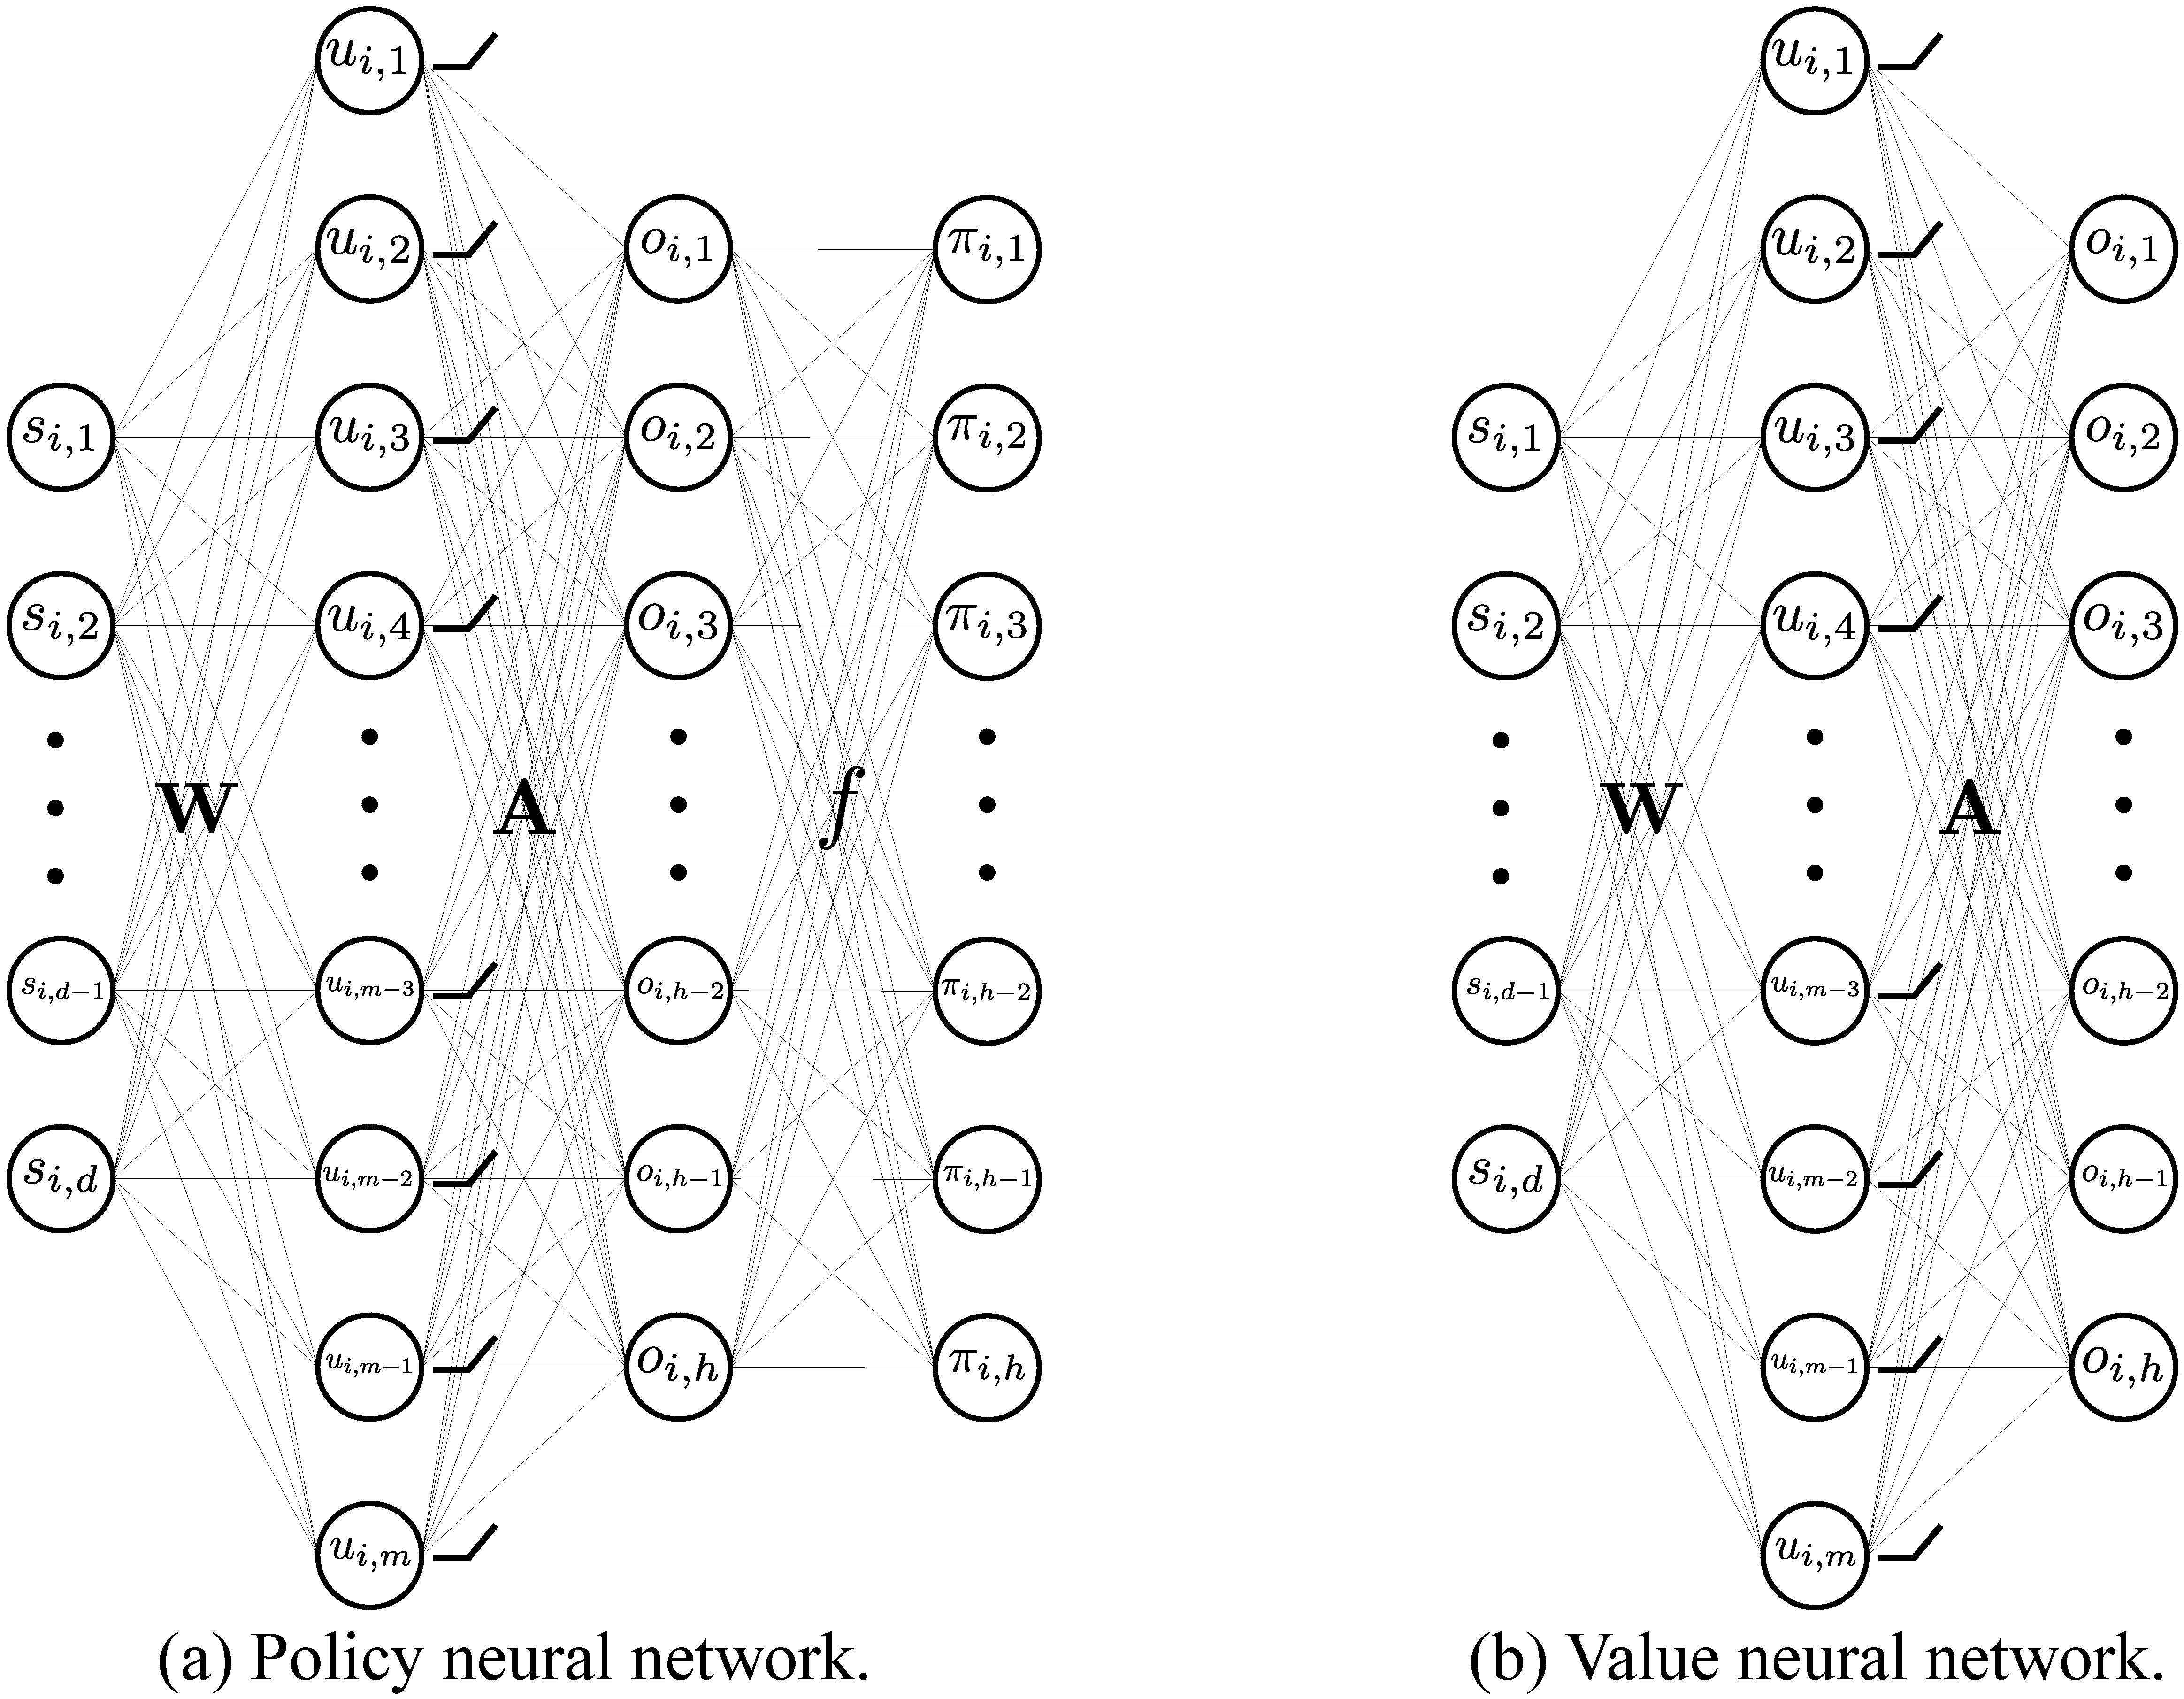
\includegraphics[width=0.9\columnwidth]{nn_policy_value_vertical.pdf}}
		\caption{The structure of the policy neural network and the value neural network.}
		\label{fig:nn_policy_value}
	\end{center}
	\vskip -0.2in
\end{figure}


\newpage

\begin{algorithm}[h]
   \caption{Policy Gradient with Uniform Exploration (PGE)}
\label{alg:policy_gradient_uniform_exploration}
\begin{algorithmic}
   \STATE {\bfseries Input:} State feature $\rvs$, learning rate $\eta > 0$, $\beta > 0$.
   \STATE $\rvw_r(0) \sim \gN\left( 0, \sigma^2 \cdot \rmI \right)$, $\forall r \in [m]$. $a_{k, r} \sim 
   \unif\left\{-1, +1\right\}$, $\forall k \in [h]$, $\forall r \in [m]$.
   \STATE $\hat{r}_{0}(k) \gets 0$, $n_{0}(k) \gets 0$, $\tilde{\pi}_0(k) \gets \frac{1}{h}$, $\forall k \in [h]$.
   \FOR{$t=0$ {\bfseries to} $T-1$}
   \STATE Sample action $A_{t} \sim \tilde{\rvpi}_{t}\left(\cdot \middle| \rvs \right)$. Take action $A_{t}$. Observe reward $R_{ A_{t}}\left(n_{t}\left(A_t\right) \right)$.
   \STATE $\rmW_{t+1} \leftarrow \rmW_t + \eta \cdot \frac{d \rvpi\left(\rmW_t\right)^\top \hat{\rvr}_t}{d \rmW_t}$.
   \STATE $n_{t+1}(k) \gets \left. 
		\begin{cases}
		n_{t}(k) + 1, & \text{if } k = A_t, \\
		n_{t}(k), & \text{otherwise}.
		\end{cases}
		\right. \qquad$ 
   $\hat{r}_{t+1}(k) \gets \left. 
		\begin{cases}
		\frac{n_{t}(k) \cdot \hat{r}_{t}(k) + R_{k}\left(n_{t}(k)\right) }{n_{t+1}(k)}, & \text{if } k = A_t, \\
		\hat{r}_{t}(k), & \text{otherwise}.
		\end{cases}
		\right.$
   \STATE $\tilde{\pi}_{t+1}(k) \gets \left( 1 - \left(t+1\right)^{ \beta - \frac{1}{3}} \right) \cdot \pi\left(\rmW_{t+1}\right)(k) + \left(t+1\right)^{ \beta - \frac{1}{3}} \cdot \frac{1}{h}$, $\forall k \in [h]$.
   \ENDFOR
\end{algorithmic}
\end{algorithm}

\begin{algorithm}[h]
	\caption{Logit Learning with $\varepsilon$-Greedy Exploration (LLE)}
	\label{alg:logit_learning_eps_greedy_exploration}
	\begin{algorithmic}
		\STATE {\bfseries Input:} State feature $\rvs$, $\eta > 0$, $\alpha > 0$, $\beta > 0$.
		\STATE $\rvw_r(0) \sim \gN\left( 0, \sigma^2 \cdot \rmI \right)$, $\forall r \in [m]$. $a_{k, r} \sim \unif\left\{-1, +1\right\}$, $\forall k \in [h]$, $\forall r \in [m]$.
		\STATE $\hat{r}_{0}(k) \gets 0$, $n_{0}(k) \gets 0$, $\tilde{\pi}_t(k) \gets \frac{1}{h}$, $\ucb_{0}(k) \gets 1$, $\lcb_{0}(k) \gets 0$, $\forall k \in [h]$.
		\STATE Take every action $k$ once, update $n_{0}(k)$ and $\hat{r}_{0}(k)$.
		\FOR{$t=0$ {\bfseries to} $T-1$}
		
		\STATE Sample action $A_{t} \sim \tilde{\rvpi}_t\left(\cdot \middle| \rvs \right)$. Take action $A_{t}$. Observe reward $R_{ A_{t}}\left(n_{t}\left(A_t\right) \right)$.
		\STATE $\rmW_{t+1} \leftarrow \rmW_t - \eta \cdot \frac{d \left\{ \frac{1}{2} \left\| \rvo\left( \rmW_t\right) - \hat{\rvr}_t \right\|_2^2 \right\}}{d \rmW_t}$.
		\STATE $n_{t+1}(k) \gets \left. 
		    \begin{cases}
		    n_{t}(k) + 1, & \text{if } k = A_t, \\
		    n_{t}(k), & \text{otherwise}.
		    \end{cases}
		    \right. \qquad$
		%\STATE $n_{t+1}\left(A_t\right) \gets n_{t}\left(A_t\right) + 1$.
		%\STATE $n_{t+1}(k) \gets n_{t}(k)$, $\forall k \not= A_t$.
		$\hat{r}_{t+1}(k) \gets \left. 
		    \begin{cases}
		    \frac{n_{t}(k) \cdot \hat{r}_{t}(k) + R_{k}\left(n_{t}(k)\right) }{n_{t+1}(k)}, & \text{if } k = A_t, \\
		    \hat{r}_{t}(k), & \text{otherwise}.
		    \end{cases}
		    \right.$
		%\STATE $\hat{r}_{t+1}\left(A_t\right) \gets \frac{n_{t}\left(A_t\right) \cdot \hat{r}_{t}\left(A_t\right) + R_{A_{t}}\left(n_{t}\left(A_t\right)\right) }{n_{t+1}\left(A_t\right)}$.
		%\STATE $\hat{r}_{t+1}(k) \gets \hat{r}_{t}(k)$, $\forall k \not= A_t$.
		\STATE $\ucb_{t+1}(k) \gets
		    \min{\left\{ 1, \hat{r}_{t+1}(k) + \sqrt{\frac{\alpha \ln{\left( (t+1) h^{\frac{1}{\alpha}}\right)}}{2 n_{t+1}(k)}}\right\}}$, $\forall k \in [h]$.
		%\STATE $\ucb_{t+1}\left(A_t\right) \gets \min{\left\{ 1, \hat{r}_{t+1}\left(A_t\right) + \sqrt{\frac{\alpha \ln{\left( t h^{\frac{1}{\alpha}}\right)}}{2 n_{t+1}\left(A_t\right)}}\right\}}$.
		%\STATE $\ucb_{t+1}(k) \gets \ucb_{t}(k)$, $\forall k \not= A_t$.
		\STATE $\lcb_{t+1}(k) \gets 
		    \max{\left\{ 0, \hat{r}_{t+1}(k) - \sqrt{\frac{\alpha \ln{\left( t h^{\frac{1}{\alpha}}\right)}}{2 n_{t+1}(k)}}\right\}}$, $\forall k \in [h]$.
		%\STATE $\lcb_{t+1}\left(A_t\right) \gets \max{\left\{ 0, \hat{r}_{t+1}\left(A_t\right) - \sqrt{\frac{\alpha \ln{\left( t h^{\frac{1}{\alpha}}\right)}}{2 n_{t+1}\left(A_t\right)}}\right\}}$.
		%\STATE $\lcb_{t+1}(k) \gets \lcb_{t}(k)$, $\forall k \not= A_t$.
		
		\STATE $\hat{\Delta}_{t+1}(k) \gets \min\left\{ 1,  \min\limits_{k^\prime \in \left[h\right]}\left\{ \lcb_{t+1}(k^\prime) \right\}  - \ucb_{t+1}(k)\right\} $, $\forall k \in [h]$.
		\STATE $\xi_{t+1}(k) \gets \frac{\beta \ln{(t+1)}}{(t+1) \hat{\Delta}_{t+1}^2(k)}$, $\varepsilon_{t+1}(k) \gets \min\left\{ \frac{1}{2 h}, \frac{1}{2} \sqrt{\frac{\ln{h}}{(t+1) h}},  \xi_{t+1}(k) \right\}$, $\forall k \in [h]$.
		\STATE $\pi_{t+1}(k) \gets \left. 
		    \begin{cases}
		    1, & \text{if } k = \argmax\limits_{k^\prime \in \left[h\right]}\left\{ o_{t+1}(k^\prime)\right\}, \\
		    0, & \text{otherwise}.
		    \end{cases}
		    \right.$
		%\STATE $\pi_{t}(k) \gets 1$, for $k = \argmax\limits_{k^\prime \in \left[h\right]}\left\{ o_{t}(k^\prime)\right\}$.
		%\STATE $\pi_{t}(k) \gets 0$, $\forall k \not= \argmax\limits_{k^\prime \in \left[h\right]}\left\{ o_{t}(k^\prime)\right\}$.
		\STATE $\tilde{\pi}_{t+1}(k) \gets \left( 1 - \sum\limits_{k^\prime \in [h]}{\varepsilon_{t+1}(k)} \right) \cdot  \pi_{t+1}(k) + \varepsilon_{t+1}(k)$, $\forall k \in [h]$.
		
		\ENDFOR
	\end{algorithmic}
\end{algorithm}

\end{document}